% ALGUNOS PAQUETES REQUERIDOS (EN UBUNTU): %
% ========================================
% %
% texlive-latex-base %
% texlive-latex-recommended %
% texlive-fonts-recommended %
% texlive-latex-extra %
% texlive-science %
% texlive-lang-spanish (en ubuntu 13.10) %
% ******************************************************** %

\documentclass[a4paper]{article}
\usepackage[spanish]{babel}
\usepackage[utf8]{inputenc}
\usepackage{fancyhdr}
\usepackage[pdftex]{graphicx}
\usepackage{sidecap}
\usepackage{caption}
\usepackage{subcaption}
\usepackage{booktabs}
\usepackage{makeidx}
\usepackage{float}
\usepackage{amsmath, amsthm, amssymb}
\usepackage{amsfonts}
\usepackage{sectsty}
\usepackage{wrapfig}
\usepackage{listings}
\usepackage{pgfplots}
\usepackage{enumitem}
\usepackage{hyperref}
\usepackage{listings}
\usepackage{listingsutf8}

\linespread{factor}

\definecolor{mygreen}{rgb}{0,0.6,0}
\definecolor{mygray}{rgb}{0.5,0.5,0.5}
\pgfplotsset{compat=1.3}
\setlist[enumerate]{label*=\arabic*.}
\lstset{
	inputencoding=utf8/latin1,
	language=C++,
	basicstyle=\ttfamily,
	keywordstyle=\bfseries\color{blue},
	stringstyle=\color{red}\ttfamily,
	commentstyle=\color{mygreen}\ttfamily,
	morecomment=[l][\color{magenta}]{\#},
	numbers=left,
	numberstyle=\color{mygray}
}

\usepackage{color} % para snipets de codigo coloreados
\usepackage{fancybox}  % para el sbox de los snipets de codigo

\definecolor{litegrey}{gray}{0.94}

% \newenvironment{sidebar}{%
% 	\begin{Sbox}\begin{minipage}{.85\textwidth}}%
% 	{\end{minipage}\end{Sbox}%
% 		\begin{center}\setlength{\fboxsep}{6pt}%
% 		\shadowbox{\TheSbox}\end{center}}
% \newenvironment{warning}{%
% 	\begin{Sbox}\begin{minipage}{.85\textwidth}\sffamily\lite\small\RaggedRight}%
% 	{\end{minipage}\end{Sbox}%
% 		\begin{center}\setlength{\fboxsep}{6pt}%
% 		\colorbox{litegrey}{\TheSbox}\end{center}}

\newenvironment{codesnippet}{%
	\begin{Sbox}\begin{minipage}{\textwidth}\sffamily\small}%
	{\end{minipage}\end{Sbox}%
		\begin{center}%
		\vspace{-0.4cm}\colorbox{litegrey}{\TheSbox}\end{center}\vspace{0.3cm}}



\usepackage{fancyhdr}
\pagestyle{fancy}
%\renewcommand{\chaptermark}[1]{\markboth{#1}{}}
\renewcommand{\sectionmark}[1]{\markright{\thesection\ - #1}}
\fancyhf{}
\fancyhead[LO]{\rightmark} % \thesection\
\fancyfoot[LO]{\small{Franco Frizzo, Iván Pondal, Manuel Mena, Maximiliano León Paz}}
\fancyfoot[RO]{\thepage}
\renewcommand{\headrulewidth}{0.5pt}
\renewcommand{\footrulewidth}{0.5pt}
%\setlength{\hoffset}{-0.8in}
\setlength{\textwidth}{16cm}
\setlength{\hoffset}{-1.1cm}
\setlength{\headsep}{0.5cm}
\setlength{\textheight}{25cm}
\setlength{\voffset}{-0.7in}
\setlength{\headwidth}{\textwidth}
\setlength{\headheight}{13.1pt}
\renewcommand{\baselinestretch}{1.1} % line spacing

\usepackage{caratula}

\newcommand{\ord}{\ensuremath{\operatorname{O}}}
\newcommand{\nat}{\ensuremath{\mathbb{N}}}
\newcommand{\acr}[1]{\lowercase{\textsc{#1}}}
\newcommand{\comp}{\ensuremath{^{\operatorname{C}}}}
\newcommand{\argmax}{\operatornamewithlimits{arg\,m\acute{a}x}}

% Lemas, definiciones, etc.
\theoremstyle{plain}
  \newtheorem{prop}{Proposición}
  \newtheorem{lema}{Lema}
\theoremstyle{remark}
  \newtheorem{obs}{Observación}
\theoremstyle{definition}
  \newtheorem{defi}{Definición}

% Pseudocódigo
\usepackage[onelanguage, spanish]{algorithm2e}
    % \NoCaptionOfAlgo
    \LinesNumbered\RestyleAlgo{ruled}\IncMargin{1em}\DontPrintSemicolon\SetArgSty{}\SetCommentSty{textsf}\SetFuncSty{textsf}
    \SetKwInput{Input}{Entrada}
    \SetKwInput{Output}{Salida}
    \SetKwProg{For}{para}{ hacer}{fin}
    \SetKwProg{Fn}{función}{:}{fin}

%\lstset{
%    language=C++,
%    basicstyle=\ttfamily,
%    keywordstyle=\color{blue}\ttfamily,
%    stringstyle=\color{red}\ttfamily,
%    commentstyle=\color{ForestGreen}\ttfamily,
%    morecomment=[l][\color{magenta}]{\#}
%}

\begin{document}
\materia{Algoritmos y Estructuras de Datos III}
\submateria{Primer cuatrimestre de 2016}
\titulo{Trabajo Práctico III}
%\subtitulo{Grupo: }
\integrante{Franco Frizzo}{013/14}{francofrizzo@gmail.com}
\integrante{Iván Pondal}{078/14}{ivan.pondal@gmail.com}
\integrante{Manuel Mena}{313/14}{manuelmena1993@gmail.com}
\integrante{Maximiliano León Paz}{251/14}{m4xileon@gmail.com}

\maketitle
% no footer on the first page
\thispagestyle{empty}

\newpage
\tableofcontents

% Mostrar paper principal en bibliografía aunque no sea citado
\nocite{ehrlich}

\newpage
\setcounter{secnumdepth}{0}
\section{Introducción}
\setcounter{secnumdepth}{1}


\newpage
\section{Ejercicio 1: Aplicaciones del problema en la ciencia molecular}

% El Doc ha estudiado este problema durante mucho tiempo, y cree entender que
% se puede resolver gracias a las aplicaciones prácticas de la teoría de
% grafos que describen en su paper Ehrlich y Rarey [1]. Está convencido de que
% con resolver MCS le alcanza para rediseñar correctamente la nueva componente
% en cuestión, pero Marty desconfía.
% a) Su tarea consiste en leer este paper y explicarle a Marty qué problema de
%    grafos se buscar resolver en las aplicaciones del paper, encontrar las
%    diferencias entre dicho problema y MCS, y explicar qué aplicaciones tiene
%    este problema en la química. No es parte de este TP resolver el problema
%    del paper, en todo caso es problema del Doc.

Entre las diversas aplicaciones que tiene el problema de \acr{MCS}, cabe
destacar las relacionadas con el campo de la química y la biología molecular,
en las que pone el foco el trabajo de Ehrlich y Rarey\cite{ehrlich}. Los
grafos constituyen una forma muy conveniente e intuitiva de representar la
estructura de una molécula, con la ventaja agregada de poder aprovechar el
gran conocimiento computacional existente sobre el tema. En este contexto,
resolver el problema de \acr{MCS} resulta de gran utilidad para buscar
subestructuras comunes entre dos moléculas dadas, o cuantificar la similitud
entre las mismas.

El artículo engloba, bajo el nombre general de \acr{MCS}, a dos problemas
similares, denominados \acr{MCES} (\emph{maximum common edge subgraph}) y
\acr{MCIS} (\emph{maximum common induced subgraph}). El primero de ellos
coincide con el problema que se estudiará en este trabajo: dados dos grafos,
encontrar el subgrafo común a ambos con máxima cantidad de aristas. El
segundo, en cambio, consiste en encontrar un grafo con la mayor cantidad
posible de nodos que sea isomorfo, simultáneamente, a un subgrafo inducido de
otros dos grafos.

Dentro del contexto de aplicación estudiado por el paper, los grafos
utilizados presentan ciertas particularidades. Con frecuencia, al modelar
estructuras moleculares, se utilizan etiquetas para indicar propiedades de los
átomos o enlaces representados por cada uno de los nodos o aristas,
respectivamente. Luego, cuando se desea resolver \acr{MCS} para encontrar
subestructuras comunes a dos moléculas, solo pueden mapearse átomos o enlaces
cuyas etiquetas coincidan, agregando una nueva restricción al problema que no
está presente en la versión que será abordada en este trabajo.

En el trabajo citado, se hace un recorrido por diversos escenarios en los que
resulta aplicable \acr{MCS}, la mayoría de ellos en el área de la biología
molecular. Se mencionan dos grandes categorías de problemas: los relacionados
con pequeñas moléculas orgánicas, como las drogas, y los concernientes a
moléculas grandes, por ejemplo, las proteínas. Algunos de los incluidos en el
primer grupo son la obtención de métricas de similitud estructural que
permiten la clasificación de compuestos en familias o la predición de sus
efectos activos, el mapeo de átomos y enlaces entre reactivos y productos en
reacciones, y la elaboración de modelos matemáticos para cuantificar
la relación entre estructura y la actividad de compuestos químicos. En el
segundo grupo, se puede mencionar tanto la búsqueda de semejanzas
estructurales entre moléculas a escala global como la identificación de
similitudes de carácter local; estas útimas resultan de utilidad para procesar
grandes bases de datos y elaborar hipótesis acerca del origen evolutivo y las
funciones desempeñadas por las proteínas.


\newpage
\section{Algoritmo exacto para el caso general}

% Para convencer a Marty, el Doc necesita mostrarle un algoritmo que
% efectivamente resuelva el problema. Dado que sus habilidades de programador
% están un poco oxidadas, se les pide diseñar e implementar un algoritmo
% exacto para MCS y desarrollar los siguientes puntos que justifiquen la
% solución encontrada:
% a) Explicar detalladamente el algoritmo implementado. Elaborar podas y
%    estrategias que permitan mejorar los tiempos de resolución.
% b) Calcular el orden de complejidad temporal de peor caso del algoritmo.
% c) Realizar una experimentación que permita observar los tiempos de
%    ejecución del algoritmo en función del tamaño de entrada y de las podas
%    y/o estrategias implementadas.

\subsection{Introducción}
En este ejercicio, se busca encontrar un algoritmo exacto para resolver, en
tiempo exponencial, el problema del \acr{MCS} entre dos grafos cualquiera.
Para ello, se utiliza la técnica de \textit{backtracking}. Este método es
extremadamente costoso tanto temporal como espacialmente, por lo que no solo
es recomendable sino necesario realizar podas y estrategias que
permitan mejorar los tiempos de resolución.

\subsection{Resolución}
El algoritmo consiste en probar todos los mapeos posibles entre los nodos de
ambos grafos, y así tomar un grafo común con la mayor cantidad de aristas de
entre todas las combinaciones de mapeos.

Dentro de la función principal, aquella que emplea la técnica de
\textit{backtracking}, se hace uso de ambos grafos, otro grafo que representa
el subgrafo común máximo dentro de la rama actual de ejecución (inicialmente
vacío), dos listas enlazadas (una para cada grafo) que contienen
los IDs de los nodos aún no mapeados en esta rama de ejecución, y un mapa
implementado sobre una tabla de \emph{hash} que contiene los mapeos hechos en esa
rama de ejecución.

\vspace{1em}

\begin{algorithm}[H]
    \SetAlgoVlined
    \caption{\acr{MCS} exacto, utilizando \emph{backtracking}}
    \label{algo:backtracking}

    \Input{Dos grafos $g_1$ y $g_2$ donde los nodos se representan con enteros,
    el subgrafo común máximo de esta rama de ejecución $mcs$ pasado por
    referencia (cada nodo en este subgrafo consiste de un par de enteros que
    representa el mapeo entre nodos de $g_1$ y $g_2$, dos listas enlazadas
    $l_1$ y $l_2$ y un mapa $mapeos$.}
    \Output{Un booleano que indica si el subgrafo pasado por referencia es
    válido (para más adelante efectuar podas).}

    \If {$l_1$.vacia() $\lor$ $l_2$.vacia()} {
        \Return{verdadero}
    }

    $maxMCS$ $\gets$ grafo de pares vacío \;

    \For {$nodo_1 \in l_1$} {
        \For {$nodo_2 \in l_2$} {

            $l_1$.borrar($nodo_1$) \;
            $l_2$.borrar($nodo_2$) \;

            $copiaMapeos$ $\gets$ $mapeos$ \;
            $copiaMapeos$.insertar($nodo_1$, $nodo_2$) \;

            $copiaMCS$ = $mcs$.clonar() \;
            $copiaMCS$.agregarNodo(par($nodo_1$, $nodo_2$)) \;

            \For {$vecino \in g_1$.vecinos($nodo_1$)} {
                $mapeadoAVecino$ $\gets$ $mapeos$.valor($vecino$) \;
                \If {$mapeos$.esta($vecino$) $\land g_2$.adyacentes($nodo_2$,
                $mapeadoAVecino$) } {
                    $copiaMCS$.agregarEje(par($nodo_1$, $nodo_2$), par($vecino$,
                    $mapeadoAVecino$))
                }
            }

            MCSBacktracking($g1$, $g2$, $copiaMCS$, $copiaMapeos$, $l_1$, $l_2$) \;

            \If {$MCSBacktraking$ es valido $\land copiaMCS$.m() $\geq maxMCS$.m()} {
                $maxMCS$ $\gets$ $copiaMCS$ \;
            }

            $l_1$.reinsertar($nodo_1$) \;
            $l_2$.reinsertar($nodo_2$) \;
        }
    }

    $mcs$ $\gets$ $maxMCS$

    \Return{verdadero}
\end{algorithm}

\vspace{1em}

Lo que se expone en el Algoritmo \ref{algo:backtracking} es el pseudocódigo
del algoritmo principal. Por simplicidad, se omiten momentáneamente las podas
del algoritmo; posteriormente se ahondará en ellas.

Se iteran $l_1$ y $l_2$
mediante dos ciclos anidados para, de esta forma, probar todos los elementos de
$l_1$ contra todos los de $l_2$ formando todos los pares de nodos posibles.
Dentro de la doble iteración se prueba el mapeo de los dos nodos seleccionados
actualizando las listas de nodos restantes y el mapa, y se hace el llamado
recursivo pasando una copia del \textit{mcs} por referencia, al cual se le
añade previamente un nodo que representa el mapeo.

Una vez terminados los ciclos se le asigna la mayor de las copias de
\textit{mcs} al subgrafo pasado por referencia.

\subsubsection{Podas y optimizaciones}

Se puede apreciar en el pseudocódigo anterior la existencia de una condición
para asignar el \textit{mcs} obtenido a la variable que almacena el máximo de
las iteraciones tras el llamado recursivo (además de la que verifica si es
su cantidad de aristas es mayor). Se pide que el resultado del llamado haya sido
válido, que es lo mismo que pedir que el valor retornado por la misma sea
verdadero. Esto podría parecer no tener sentido, ya que en todos los casos el valor
devuelto es verdadero, pero la razón de esto es que no están incluidas las podas. La
forma de podar el árbol de ejecución que utilizamos hace uso de esa condición;
si se decide cortar la rama de ejecución entonces se devuelve falso y esta
estructura evitará chequeos innecesarios.

Las podas implementadas fueron las siguientes:

\begin{enumerate}
\item Verificar que la suma de los grados de los nodos que aún no han sido
mapeados pueda ser mayor que la máxima cantidad de aristas alcanzada hasta
el momento. De no ser así, se detiene y se corta la rama que está siendo
explorada.
\item Evitar armar grafos donde las permutaciones de mapeos representan el
mismo grafo.
\end{enumerate}

La verificación de la suma de los grados es sencilla. Consiste en recorrer la
lista de nodos restantes e ir sumando los grados de cada uno de ellos. Si esa
suma junto con la cantidad de ejes del \textit{mcs} actual no puede superar
a la cantidad de ejes del máximos \textit{mcs} alcanzado en alguna de las
ramas de la ejecución previamente visitadas, entonces no tiene sentido seguir
porque no es posible llegar a una mejor solución, por lo que se corta la
ejecución.

Para esto se hace uso de una estructura condicional que termina el llamado
devolviendo falso. Esta estructura es lo primero que se ejecuta cuando se hace
el llamado recursivo. A continuación puede verse el pseudocódigo de la poda.

\begin{algorithm}
    \SetAlgoVlined
    \caption{Poda: suma de grados}
    \If {$mcs$.m() + sumaDeGrados($l_1$) $\leq$ $maximaCantEjes$} {
        \Return{falso}
    }
\end{algorithm}

$maximaCantEjes$ es una referencia a una variable que es pasada por parámetro
en el llamado recursivo y que se actualiza si se encuentra un mejor
\textit{mcs}.

La otra poda se enfoca en evitar inspeccionar una solución cuya rama de
ejecución es equivalente a una visitada anteriormente. A modo de ejemplo, sean
los grafos $A$ y $B$ con nodos $a_1, ..., a_n$ y $b_1, ..., b_k$. Durante la
ejecución del algoritmo se mapearán todas las posibles combinaciones entre
los nodos de estos grafos. Al mapearlos hay un orden que intrínsecamente
determina cual es el mejor grafo en común, es decir, según que par de nodos
se mapeen, en el siguiente llamado recursivo el mapeo de otros dos nodos
será más eficiente o no en cuestión de cantidad de aristas del \textit{mcs}.
Pero aún así, cuando el conjunto de pares de nodos mapeados es el mismo (esto
aplica para cualquier momento del algoritmo, no necesariamente tienen que
haber sido mapeados todos los nodos) puede ser permutado y el \textit{mcs}
entre los grafos será el mismo, puesto que los nodos elegidos son los mismos.
Por esto es que la intención de esta poda es evitar llegar a un grafo con el
mismo conjunto de nodos mapeados, para así ahorrar llamados.

A continuación puede verse la imagen de un ejemplo de dos grafos junto con el
árbol de mapeos que se forma, ilustrando la idea.

\begin{center}
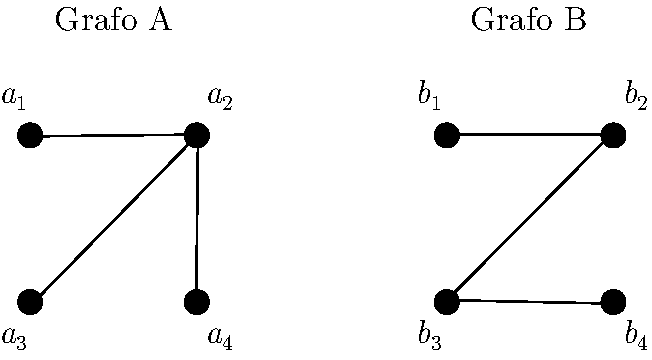
\includegraphics[width=.45\textwidth]{imagenes/ex2_grafos.pdf}
\end{center}

Las ramas en rojo son equivalentes, es decir, que representan la formación de
subgrafos comunes máximos isomorfos.

\begin{center}
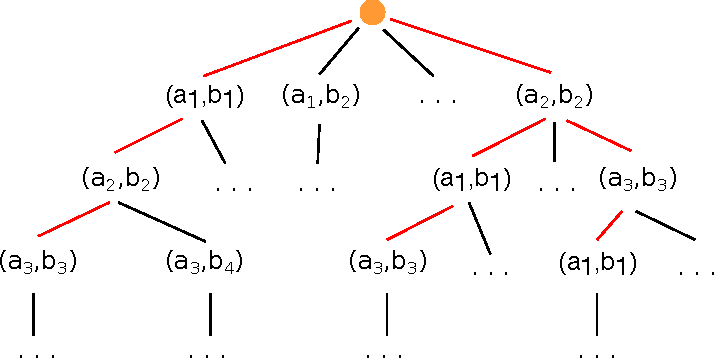
\includegraphics[width=.7\textwidth]{imagenes/ex2_execution_tree.pdf}
\end{center}

Para lograr esto utilizamos una referencia a una variable que es pasada por
parámetro en el llamado recursivo que almacena conjuntos de pares. La idea es
que antes de hacer un llamado recursivo se busque dentro de este conjunto
si el actual conjunto de mapeos ya ha sido visitado. De ser así entonces no se
hace el llamado sino que continúa la iteración, formando un nuevo par para ser
mapeado en lugar del que ha sido rechazado.

El problema con esta idea es que tiene un costo temporal demasiado alto, al
punto de representar una desventaja, ya que la comparación entre dos conjuntos
implica gran cantidad de operaciones, y esto hay que hacerlo con todos los
conjuntos de pares del mismo cardinal. A medida que la cantidad de nodos
mapeados aumenta, se vuelve más costoso, y a su vez, menos provechoso debido
a que al llegar a un nivel más profundo en la rama de ejecución, la cantidad
de llamados que pueden ser omitidos es menor.

Por esta razón, se decidió hacer efectiva esta poda únicamente para el segundo
nivel del árbol de ejecución. De esta forma las estructuras posibles se
simplifican lo suficiente como para requerir una baja complejidad temporal;
además, es el nivel en el que más ramas pueden descartarse.

La implementación de esta poda se realiza dentro del ciclo anidado, justo
después de haber elegido los nodos candidatos a ser mapeados. A continuación
puede verse el pseudocódigo de la poda.

\begin{algorithm}
    \SetAlgoVlined
    \caption{Poda: permutaciones}
    \If {$mcs$.n() == 1} {
        $permutacion$ $\gets$ tupla con el primer par mapeado y el par actual \;
        \If {$permutaciones$.esta($permutacion$)} {
            romper el ciclo \;
        }
        \Else {
            $permutaciones$.guardar($permutacion$) \;
        }
    }
\end{algorithm}

$permutaciones$ es un conjunto implementado sobre un conjunto de \emph{hash}.

La cantidad de hojas del árbol de ejecución que se ahorran es igual al
producto entre la cantidad de mapeos posibles en cada nivel, desde el tercero
hasta el último. La cantidad de mapeos posibles en un nivel es igual al
producto entre la cantidad de nodos restantes de cada grafo. Entonces, la
cantidad de hojas ahorradas es igual a $(N_1 - 2) \times (N_2 - 2) \times
(N_1 - 3) \times (N_2 - 3) \times \dots \times 1 \times (N_2 - N_1 + 1)$ si
suponemos que el segundo grafo es mayor o igual que el primero. Esto es
equivalente a $\frac{(N_1 - 2)! \times (N_2 - 2)!}{(N_2 - N_1)!}$, por lo que
fácilmente puede apreciarse por qué esta poda resulta buena.

En un principio se pensó que estas podas no resultarían demasiado efectivas,
dudando incluso de si el costo de cada una no podría significar una
desmejora en relación a la ganancia. No obstante, ambas podas no solo
acabaron siendo muy buenas, sino incluso fundamentales a medida que el tamaño de los
grafos crecía.

\subsection{Complejidad}

Para medir la complejidad del algoritmo, en principio, se analizará el
árbol de ejecución dado por el mismo. Se definen $N_1$ y $N_2$, las cantidades
de nodos de los grafos, y se supone $N_1 \leq N_2$. Por cada llamado de
la función, se hace una cantidad de llamados recursivos que depende de en qué
nivel del árbol de ejecución se encuentre actualmente el algoritmo. Esto es
así debido a que el llamado recursivo se encuentra dentro del ciclo anidado,
y la cantidad de iteraciones de ese ciclo depende de la cantidad de nodos que
aún no han sido mapeados. Como en cada llamado se mapea un par de nodos, la
cantidad de nodos por mapear va disminuyendo en cada nivel.

Para el nivel $i$ la cantidad de veces que se hace el llamado es de
$(N_1 - i)  (N_2 - i)$, que es resultado de probar todos los posibles
pares entre los nodos restantes de ambos grafos. De esta forma, la cantidad de
llamados en un nivel es de
$\frac{N_1!  N_2!}{(N_1 - i)!  (N_2 - i)!}$.

Ahora se hará foco en la complejidad del algoritmo en para cada nivel $i$.

\begin{itemize}
\item Se recorren linealmente los nodos restantes para saber si es posible
efectuar la poda de la suma de grados. $\ord(N_1 - i)$.
\item Dentro del doble ciclo anidado que se ejecuta
$(N_1 - i)  (N_2 - i)$ veces
    \begin{itemize}
    \item Copiar el mapa. $\ord(i)$.
    \item Clonar subgrafo. $\ord(i)$
    \item Agregar nodo. $\ord(i)$
    \item Agregar ejes al nuevo nodo del \acr{MCS}. Lineal sobre la cantidad de
    vecinos del nuevo nodo.
    \item Mover iteradores hasta la posición correspondiente.
    $\ord(N_1 - i + N_2 - i)$
    \end{itemize}

    Entones, el doble ciclo tiene complejidad

    \begin{align*}
    \sum_{k = 1}^{N_1 - i} \sum_{j = 1}^{N_2 - i} (\ord(i) + & \ord(\deg(v_{kj}) +
     \ord(N_1 + N_2 - 2i)) \\
    =& \sum_{k = 1}^{N_1 - i} \sum_{j = 1}^{N_2 - i} (\ord(\deg(v_{kj}) +
     \ord(N_1 + N_2)) \\
    =& \ord((N_1 - i)  (N_2 - i)  (N_1 + N_2)) + \sum_{k = 1}^{N_1 - i}
     \sum_{j = 1}^{N_2 - i} \ord(\deg(v_{kj}))
    \end{align*}

    Puede acotarse superiormente el grado de $v_{kj}$ por $N_1$, ya que no puede
    tener más de $N_1 - 1$ vecinos. Entonces, la complejidad es

    \begin{align*}
    \ord((N_1 - i) & (N_2 - i)  (N_1 + N_2)) + \sum_{k = 1}^{N_1 - i}
    \sum_{j = 1}^{N_2 - i} \ord(N_1) \\
    =& \ord((N_1 - i)  (N_2 - i)  (N_1 + N_2)) + \ord((N_1 - i)
    (N_2 - i)  N_1) \\
    =& \ord((N_1 - i)  (N_2 - i)  (N_1 + N_2 + N_1)) \\
    =& \ord((N_1 - i)  (N_2 - i)  (N_1 + N_2))
    \end{align*}

\end{itemize}

Por lo tanto la complejidad en el nivel $i$ es $\ord(N_1 - i) +$
$\ord((N_1 - i)  (N_2 - i)  (N_1 + N_2)) = \ord((N_1 - i) $
$ (N_2 - i)  (N_1 + N_2))$.

La cantidad de niveles que tiene el árbol de ejecución es $N_1$, ya que se
hacen llamados recursivos hasta que uno de los grafos tenga todos sus nodos
mapeados. Como se vio anteriormente, en cada nivel se hacen
$\frac{N_1!  N_2!}{(N_1 - i)!  (N_2 - i)!}$ llamados, por lo que
la cantidad total de llamados es de
$\sum_{i = 0}^{N_1} \frac{N_1!  N_2!}{(N_1 - i)!  (N_2 - i)!}$.

Puede acotarse esta cantidad de llamados superiormente de modo que sea
$\ord \left(N_1  \frac{N_1!  N_2!}{(N_2 - N_1)!} \right)$ siendo $N_1$ la
cantidad de niveles y $\frac{N_1!  N_2!}{(N_2 - N_1)!}$ la de hojas.

\vspace{1em}

Entonces, la complejidad total del algoritmo es

\begin{multline*}
\sum_{i = 0}^{N_1}\left[\frac{N_1!  N_2!}{(N_1 - i)!  (N_2 - i)!}
\ord((N_1 - i)  (N_2 - i)  (N_1 + N_2))\right] \\
= \ord\left(N_1  \frac{N_1!  N_2!}{(N_2 - N_1)!})
\sum_{i = 0}^{N_1}\ord((N_1 - i)  (N_2 - i)
(N_1 + N_2)\right)
\end{multline*}

Desarrollando

\[
\sum_{i = 0}^{N_1}\ord((N_1 - i)  (N_2 - i)
 (N_1 + N_2))=
(N_1 + N_2)  \sum_{i = 0}^{N_1}\ord((N_1 - i)  (N_2 - i))
\]

Sea $j = N_1 - i$ y por consecuente $i = N_1 - j$; se verifica que

\begin{align*}
\ord((N_1 + N_2)) & \sum_{i = 0}^{N_1} \ord((N_1 - i)  (N_2 - i)) \\
=& \ord((N_1 + N_2))  \sum_{j = 0}^{N_1} (\ord(j)  (N_2 - N_1 + j)) \\
=& \ord((N_1 + N_2))  \sum_{j = 0}^{N_1} (\ord(j^2) + j  (N_2 - N_1)) \\
=& \ord((N_1 + N_2))  \ord\left(\sum_{j = 0}^{N_1} j^2 + (N_2 - N_1)  \sum_{j = 0}^{N_1} j\right) \\
=& \ord((N_1 + N_2))  \ord\left(\frac{1}{6}N_1(N_1 + 1)(2N_1 + 1) + \frac{1}{2}(N_2 - N_1)N_1(N_1 + 1)\right) \\
=& \ord((N_1 + N_2))  \ord\left(\frac{1}{6}(2N_1^3 + 3N_1^2 + N_1) + \frac{1}{2}(N_2 - N_1)(N_1^2 + N_1)\right) \\
=& \ord((N_1 + N_2))  \ord\left(\frac{1}{6}(2N_1^3 + 3N_1^2 + N_1) + \frac{1}{2}(N_1^2N_2 - N_1^3 + N_1N_2 - N_1^2)\right) \\
=& \ord((N_1 + N_2))  \ord\left(\frac{1}{6}(2N_1^3 + 3N_1^2 + N_1) + \frac{1}{6}(3N_1^2N_2 - 3N_1^3 + 3N_1N_2 - 3N_1^2)\right) \\
=& \ord((N_1 + N_2))  \ord\left(\frac{1}{6}(2N_1^3 + 3N_1^2 + N_1 + 3N_1^2N_2 - 3N_1^3 + 3N_1N_2 - 3N_1^2)\right) \\
=& \ord((N_1 + N_2))  \ord\left(\frac{1}{6}(-N_1^3 + N_1 + 3N_1^2N_2 + 3N_1N_2)\right) \\
=& \ord((N_1 + N_2))  \ord\left(\frac{1}{6}N_1(-N_1^2 + 1 + 3N_1N_2 + 3N_2)\right) \\
\end{align*}

\newpage
Al verificarse que $N_1 \geq N_2$, vale que $3N_1N_2 - N_1^2 \geq 2N_1^2$.
Entonces
\begin{align*}
\ord((N_1 + N_2))  \ord\left(\frac{1}{6}N_1(-N_1^2 + 1 + 3N_1N_2 + 3N_2)\right)
=& \ord((N_1 + N_2))  \ord\left(\frac{1}{6}N_1(2N_1N_2 + 3N_2)\right) \\
=& \ord((N_1 + N_2))  \ord(N_1^2N_2) \\
=& \ord((N_1 + N_2)  N_2  N_1^2)
\end{align*}

Finalmente, la complejidad del algoritmo es
\[
\ord\left(N_1 \frac{N_1!  N_2!}{(N_2 - N_1)!}\right) \ord((N_1 + N_2)  N_2  N_1^2) =
\ord\left(\frac{N_1!  N_2!}{(N_2 - N_1)!} (N_1 + N_2)  N_2  N_1^3\right)
\]

\subsection{Experimentación}

Una vez completada la implementación del algoritmo, se realizaron pruebas
experimentales con el fin de corroborar la cota teórica calculada para la
complejidad temporal del mismo. Como fue visto anteriormente, la complejidad
del algoritmo es
$\ord\left(\frac{N_1!  N_2!}{(N_2 - N_1)!} (N_1 + N_2)  N_2  N_1^3\right)$
siempre que valga $N_1 \leq N_2$.

Entonces sólo tiene sentido experimentar para medir la complejidad siempre
que se cumpla que $N_1 \leq N_2$. Con el fin de cubrir un amplio espectro de
la región acotada por esta condición se formularon experimentos que emplean
distintos valores para las cantidades de nodos de los grafos en cuestión.

\begin{enumerate}[label=\alph*)]
\item $N_1 = N_2$
\item $2N_1 = N_2$
\item $N_1 = C$
\end{enumerate}

A continuación se analiza la complejidad del algoritmo considerando las
cantidades de nodos descriptas previamente:

\begin{enumerate}[label=\alph*.]
\item
$\ord\left(\frac{N_1!  N_2!}{(N_2 - N_1)!} (N_1 + N_2)  N_2  N_1^3\right)$
$=\ord((N_1!)^2 N_1^5)$

\item
$\ord\left(\frac{N_1!  N_2!}{(N_2 - N_1)!} (N_1 + N_2)  N_2  N_1^3\right)$
$=\ord\left(\frac{N_1! (2N_1)!}{(2N_1 - N_1)!} (N_1 + 2N_1)  2N_1  N_1^3\right)$

\ \ \ \ \ \ \ \ \ \ \ \ \ \ \ \ \ \ \ \ \ \ \ \ \ \ \ \ \ \ \ \ \ \ \ \ \ \ \ \ 
$=\ord\left(\frac{N_1! (2N_1)!}{(N_1)!} 3N_1 2N_1  N_1^3\right)$

\ \ \ \ \ \ \ \ \ \ \ \ \ \ \ \ \ \ \ \ \ \ \ \ \ \ \ \ \ \ \ \ \ \ \ \ \ \ \ \ 
$=\ord\left((2N_1)! N_1^5\right)$

\item
$\ord\left(\frac{N_1!  N_2!}{(N_2 - N_1)!} (N_1 + N_2)  N_2  N_1^3\right)$
$=\ord\left(\frac{C! N_2!}{(N_2 - C)!} (C + N_2)  N_2  C^3\right)$

\ \ \ \ \ \ \ \ \ \ \ \ \ \ \ \ \ \ \ \ \ \ \ \ \ \ \ \ \ \ \ \ \ \ \ \ \ \ \ \ 
$=\ord\left(\frac{N_2!}{(N_2 - C)!}N_2^2\right)$
\end{enumerate}

Para evitar la interferencia en las mediciones de la morfología del grafo, se
fijó cada experimento para una familia de grafos determinada. Así, se tiene un
mayor control de las variables involucradas. Sin embargo, para verificar que
la cota teórica de complejidad no se cumple de forma accidental, sino que vale
para grafos de cualquier tipo, se probó con varias familias distintas.

Se experimento con las siguientes familias de grafos:

\begin{itemize}
\item \textit{Completos}: Grafo completo vs. grafo completo
\item \textit{Árboles}: Árbol vs. árbol
\item \textit{Ciclos}: Ciclos simple vs. ciclo simple
\item \textit{Bipartitos}: Grafo bipartito completo vs. grafo bipartito
completo
\end{itemize}

Se exponen ahora los gráficos de los resultados de las experimentaciones. Se
exhibe uno por cada relación en la cantidad de nodos de los grafos utilizados
distinta. Para cada uno de ellos se grafican los datos obtenidos de cada una
de las familias de grafos ya mencionadas junto a la cota de complejidad
calculada para cada caso, para así compararlas y poder observar que para cada
una de ellas el algoritmo cumple con la cota de complejidad calculada.

Las cotas de complejidad son multiplicadas por una constante que ajusta su
valor al de las experimentaciones como mas conveninete sea para poder apreciar
con mayor facilidad si el algoritmo cumple o no con ellas.

\newcommand\constante{1}
En la Figura \ref{fig:exp2:n_1_eq_n_2} pueden observarse los datos obtenidos
de la experimentación en el caso en que $N_1 = N_2$.

\begin{figure}[H]
    \caption{Tiempos de ejecución observados para $N_1 = N_2$.}
    \label{fig:exp2:n_1_eq_n_2}
    \centering
    \begin{tikzpicture}
        \begin{axis}[
                title={},
                xlabel={Cantidad de nodos ($N_1$)},
                ylabel={Tiempo de ejecución (nanosegundos)},
                scaled x ticks=false,
                scaled y ticks=false,
                enlargelimits=0.05,
                width=0.5\textwidth,
                height=0.5\textwidth,
                legend pos=outer north east,
                legend cell align=left,
                ymode=log
            ]
            \addplot[color=black] table[x index=0,y expr={\constante * x! * x! * x^5}]{../exp/ej2/equal_complete_vs_complete};
            \addplot[color=orange] table[x index=0,y index=1]{../exp/ej2/equal_complete_vs_complete};
            \addplot[color=blue] table[x index=0,y index=1]{../exp/ej2/equal_tree_vs_tree};
            \addplot[color=red] table[x index=0,y index=1]{../exp/ej2/equal_cycle_vs_cycle};
            \addplot[color=green] table[x index=0,y index=1]{../exp/ej2/equal_complete_bipartite_vs_complete_bipartite};

            \legend{
                $(N_1!)^2 N_1^5$,
                \textit{Completos},
                \textit{Árboles},
                \textit{Ciclos},
                \textit{Bipartitos}
            }
        \end{axis}
    \end{tikzpicture}
\end{figure}

Con la intención de lograr una mejor comparativa de los tiempos de ejecución
de cada familia de grafos con la cota de complejidad se analiza un cociente
entre cada familia y dicha cota. En la Figura
\ref{fig:exp2:n_1_eq_n_2:cociente} puede observarse este cociente, en donde se
grafica también la constante utilizada para ajustar la cota de complejidad,
que en este caso es 1.

\begin{figure}[H]
    \caption{Cociente entre los tiempos de ejecución observados para $N_1 = N_2$ y su cota de complejidad.}
    \label{fig:exp2:n_1_eq_n_2:cociente}
    \centering
    \begin{tikzpicture}
        \begin{axis}[
                title={},
                xlabel={Cantidad de nodos ($N_1$)},
                ylabel={Tiempo de ejecución (nanosegundos) / $\left((N_1!)^2 N_1^5\right)$},
                scaled x ticks=false,
                scaled y ticks=false,
                enlargelimits=0.05,
                width=0.5\textwidth,
                height=0.5\textwidth,
                legend pos=outer north east,
                legend cell align=left,
                ymode=log
            ]
            \addplot[color=black] table[x index=0,y expr={\constante}]{../exp/ej2/equal_complete_vs_complete};
            \addplot[color=orange] table[x index=0,y expr={\thisrowno{1} / (x! * x! * x^5)}]{../exp/ej2/equal_complete_vs_complete};
            \addplot[color=blue] table[x index=0,y expr={\thisrowno{1} / (x! * x! * x^5)}]{../exp/ej2/equal_tree_vs_tree};
            \addplot[color=red] table[x index=0,y expr={\thisrowno{1} / (x! * x! * x^5)}]{../exp/ej2/equal_cycle_vs_cycle};
            \addplot[color=green] table[x index=0,y expr={\thisrowno{1} / (x! * x! * x^5)}]{../exp/ej2/equal_complete_bipartite_vs_complete_bipartite};

            \legend{
                $\constante$,
                $\frac{\textit{Completos}}{(N_1!)^2 N_1^5}$,
                $\frac{\textit{Árboles}}{(N_1!)^2 N_1^5}$,
                $\frac{\textit{Ciclos}}{(N_1!)^2 N_1^5}$,
                $\frac{\textit{Bipartitos}}{(N_1!)^2 N_1^5}$
            }
        \end{axis}
    \end{tikzpicture}
\end{figure}

Es notorio como cada una de las familias de grafos utilizadas para esta
experimentación permanecen por debajo de la constante, lo cual indica entonces
que para el caso en que $N_1 = N_2$ el algoritmo cumple con la cota de
complejidad calculada, que es de orden $(N_1!)^2 N_1^5$, para cada una de
estas familias.

\renewcommand\constante{1}
Se expone ahora, en la Figura \ref{fig:exp2:2n_1_eq_n_2}, un gráfico con los
datos obtenidos de la experimentación en el caso en que $2N_1 = N_2$, junto a
la cota de complejidad para este caso que es $\ord((2N_1)! N_1^5)$.

\begin{figure}[H]
    \caption{Tiempos de ejecución observados para $2N_1 = N_2$.}
    \label{fig:exp2:2n_1_eq_n_2}
    \centering
    \begin{tikzpicture}
        \begin{axis}[
                title={},
                xlabel={Cantidad de nodos ($N_2$)},
                ylabel={Tiempo de ejecución (nanosegundos)},
                scaled x ticks=false,
                scaled y ticks=false,
                enlargelimits=0.05,
                width=0.5\textwidth,
                height=0.5\textwidth,
                legend pos=outer north east,
                legend cell align=left,
                ymode=log
            ]
            \addplot[color=black] table[x index=0,y expr={\constante * ((2 * x)! * x^5}]{../exp/ej2/lineal_complete_vs_complete};
            \addplot[color=orange] table[x index=0,y index=1]{../exp/ej2/lineal_complete_vs_complete};
            \addplot[color=blue] table[x index=0,y index=1]{../exp/ej2/lineal_tree_vs_tree};
            \addplot[color=red] table[x index=0,y index=1]{../exp/ej2/lineal_cycle_vs_cycle};
            \addplot[color=green] table[x index=0,y index=1]{../exp/ej2/lineal_complete_bipartite_vs_complete_bipartite};

            \legend{
                $(2N_1)! N_1^5$,
                \textit{Completos},
                \textit{Árboles},
                \textit{Ciclos},
                \textit{Bipartitos}
            }
        \end{axis}
    \end{tikzpicture}
\end{figure}

Al igual que en el experimento anterior, se grafica en la Figura
\ref{fig:exp2:2n_1_eq_n_2:cociente} el cociente entre los datos obtenidos y la
cota de complejidad de la experimentación para el caso en que $2N_1 = N_2$,
junto con la constante que multiplica la función descripta por la cota de
complejidad que en este caso es \constante.

\begin{figure}[H]
    \caption{Cociente entre los tiempos de ejecución observados para $2N_1 = N_2$ y su cota de complejidad.}
    \label{fig:exp2:2n_1_eq_n_2:cociente}
    \centering
    \begin{tikzpicture}
        \begin{axis}[
                title={},
                xlabel={Cantidad de nodos ($N_2$)},
                ylabel={Tiempo de ejecución (nanosegundos) / $((2N_1)! N_1^5)$},
                scaled x ticks=false,
                scaled y ticks=false,
                enlargelimits=0.05,
                width=0.5\textwidth,
                height=0.5\textwidth,
                legend pos=outer north east,
                legend cell align=left,
                ymode=log
            ]
            \addplot[color=black] table[x index=0,y expr={\constante}]{../exp/ej2/lineal_complete_vs_complete};
            \addplot[color=orange] table[x index=0,y expr={\thisrowno{1} / ((2 * x)! * x^5)}]{../exp/ej2/lineal_complete_vs_complete};
            \addplot[color=blue] table[x index=0,y expr={\thisrowno{1} / ((2 * x)! * x^5)}]{../exp/ej2/lineal_tree_vs_tree};
            \addplot[color=red] table[x index=0,y expr={\thisrowno{1} / ((2 * x)! * x^5)}]{../exp/ej2/lineal_cycle_vs_cycle};
            \addplot[color=green] table[x index=0,y expr={\thisrowno{1} / ((2 * x)! * x^5)}]{../exp/ej2/lineal_complete_bipartite_vs_complete_bipartite};

            \legend{
                $\constante$,
                $\frac{\textit{Completos}}{(2N_1)! N_1^5}$,
                $\frac{\textit{Árboles}}{(2N_1)! N_1^5}$,
                $\frac{\textit{Ciclos}}{(2N_1)! N_1^5}$,
                $\frac{\textit{Bipartitos}}{(2N_1)! N_1^5}$
            }
        \end{axis}
    \end{tikzpicture}
\end{figure}

Al igual que en el caso anterior, puede observarse como cada una de las
familias de grafos empleadas en esta experimentación permanecen por debajo de
la constante, lo cual indica entonces que para el caso en que $2N_1 = N_2$ el
algoritmo cumple con la cota de complejidad calculada de orden $(2N_1)! N_1^5$,
para cada una de estas familias.

\renewcommand\constante{5000}
\newcommand\valorFijo{4}
Finalmente, en la Figura \ref{fig:exp2:n_1_eq_fijo} pueden verse los datos
obtenidos de la experimentación en el caso en que $N_1 = C$. El valor elegido
es $C = \valorFijo$.

La razón por la cual el valor en que $C$ fue fijado sea \valorFijo es que para
valores muy chicos el algoritmo no ejecutaba demasiadas operaciones, lo cual
no hubiese sido fructuosa a raíz de la experimentación, y para valores grandes
el tiempo de ejecución es muy alto, lo suficiente como para correr durante
días. Como existe la condición de que $N_1 \leq N_2$, si se fija para $C$ un
valor muy alto, el algoritmo debera efectuar la búsqueda para un grafo con una
cantidad alta de nodos y otro con una cantidad mayor aún. Para un numero de 8
nodos por grafo el algoritmo comienza a enlentecerse mucho, entonces
se estableció $C = 4$ ya que permite una experimentación de tiempo aceptable,
y además un rango de nodos suficiente como para considerar la experimentación
representativa para valores mayores.

\begin{figure}[H]
    \caption{Tiempos de ejecución observados para $N_1 = \valorFijo$.}
    \label{fig:exp2:n_1_eq_fijo}
    \centering
    \begin{tikzpicture}
        \begin{axis}[
                title={},
                xlabel={Cantidad de nodos ($N_2$)},
                ylabel={Tiempo de ejecución (nanosegundos)},
                scaled x ticks=false,
                scaled y ticks=false,
                enlargelimits=0.05,
                width=0.5\textwidth,
                height=0.5\textwidth,
                legend pos=outer north east,
                legend cell align=left,
                ymode=log
            ]
            \addplot[color=black] table[x index=0,y expr={\constante * x! / (x - \valorFijo)! * x^2}]{../exp/ej2/fixed_complete_vs_complete};
            \addplot[color=orange] table[x index=0,y index=1]{../exp/ej2/fixed_complete_vs_complete};
            \addplot[color=blue] table[x index=0,y index=1]{../exp/ej2/fixed_tree_vs_tree};
            \addplot[color=red] table[x index=0,y index=1]{../exp/ej2/fixed_cycle_vs_cycle};
            \addplot[color=green] table[x index=0,y index=1]{../exp/ej2/fixed_complete_bipartite_vs_complete_bipartite};

            \legend{
                $\constante \frac{N_2!}{(N_2 - \valorFijo)!}N_2^2$,
                \textit{Completos},
                \textit{Árboles},
                \textit{Ciclos},
                \textit{Bipartitos}
            }
        \end{axis}
    \end{tikzpicture}
\end{figure}

Al igual que en el experimento anterior, se grafica en la Figura
\ref{fig:exp2:2n_1_eq_n_2:cociente} el cociente entre los datos obtenidos y la
cota de complejidad de la experimentación para el caso en que $2N_1 = N_2$,
junto con la constante que multiplica la función descripta por la cota de
complejidad que en este caso es \constante.
En la Figura \ref{fig:exp2:n_1_eq_fijo:cociente} puede verse el cociente entre
los datos obtenidos y la cota de complejidad de la experimentación en el caso
en que $N_1 = C$, siendo $C = \valorFijo$. También se grafica la constante que
multiplica la función descripta por la cota de complejidad que en este caso es
\constante.

\begin{figure}[H]
    \caption{Cociente entre los tiempos de ejecución observados para $N_1 = \valorFijo$ y su cota de complejidad.}
    \label{fig:exp2:n_1_eq_fijo:cociente}
    \centering
    \begin{tikzpicture}
        \begin{axis}[
                title={},
                xlabel={Cantidad de nodos ($N_2$)},
                ylabel={Tiempo de ejecución (nanosegundos) / $\left(\frac{N_2!}{(N_2 - \valorFijo)!}N_2^2\right)$},
                scaled x ticks=false,
                scaled y ticks=false,
                enlargelimits=0.05,
                width=0.5\textwidth,
                height=0.5\textwidth,
                legend pos=outer north east,
                legend cell align=left,
                ymode=log,
                xmin=4
            ]
            \addplot[color=black] table[x index=0,y expr={\constante}]{../exp/ej2/fixed_complete_vs_complete};
            \addplot[color=orange] table[x index=0,y expr={\thisrowno{1} / (x! / (x - \valorFijo)! * x^2)}]{../exp/ej2/fixed_complete_vs_complete};
            \addplot[color=blue] table[x index=0,y expr={\thisrowno{1} / (x! / (x - \valorFijo)! * x^2)}]{../exp/ej2/fixed_tree_vs_tree};
            \addplot[color=red] table[x index=0,y expr={\thisrowno{1} / (x! / (x - \valorFijo)! * x^2)}]{../exp/ej2/fixed_cycle_vs_cycle};
            \addplot[color=green] table[x index=0,y expr={\thisrowno{1} / (x! / (x - \valorFijo)! * x^2)}]{../exp/ej2/fixed_complete_bipartite_vs_complete_bipartite};

            \legend{
                $\constante$,
                \textit{Completos}$\frac{(N_2 - \valorFijo)!}{N_2! N_2^2}$,
                \textit{Árboles}$\frac{(N_2 - \valorFijo)!}{N_2! N_2^2}$,
                \textit{Ciclos}$\frac{(N_2 - \valorFijo)!}{N_2! N_2^2}$,
                \textit{Bipartitos}$\frac{(N_2 - \valorFijo)!}{N_2! N_2^2}$
            }
        \end{axis}
    \end{tikzpicture}
\end{figure}

Al observar que el algoritmo permanece por debajo de la constante para todas
las familias de grafos con las que se experimentó, se puede apreciar que
cumple con la cota de complejidad calculada para el caso en que se fija
$N_1 = C$.

\newpage
\section{Ejercicio 3}

% El nuevo problema que tienen Marty y el Doc es que ahora no se ponen de
% acuerdo en qué estructura quı́mica deben utilizar para armar el condensador
% de flujos. Marty, a partir de las propiedades atómicas, ha obtenido una
% constante n y está seguro de que la solución que están buscando debe ser un
% grafo de a lo sumo n vértices (o como él lo dice, un subgrafo de algún Kn),
% mientras que el Doc ha estudiado las caracterı́sticas moleculares e insiste
% con que debe ser un subgrafo de un cografo dado. Por las dudas, y para
% evitar más conflictos entre ellos, quieren cumplir con ambas
% especificaciones, siempre maximizando la cantidad de aristas, dado que éste
% es el punto clave para su funcionamiento dentro del condensador. Por eso les
% pedimos que los ayuden diseñando e implementando un algoritmo exacto para
% MCS que tenga complejidad temporal polinomial para el caso en el que G1 es
% un cografo y G2 es un grafo completo y desarrollen los siguientes puntos que
% avalen la solución encontrada (si estamos hablando de viajar en el tiempo,
% no hay margen de error posible):
% a) Explicar detalladamente el algoritmo implementado.
% b) Calcular el orden de complejidad temporal de peor caso del algoritmo.
% c) Realizar una experimentación que permita observar los tiempos de
%    ejecución del algoritmo en función del tamaño de entrada.

\subsection{Introducción}
En este ejercicio, se busca encontrar un algoritmo exacto para resolver, en
tiempo polinomial, el problema del \acr{MCS} entre dos grafos cuando uno de
ellos es un grafo completo y el otro es un \emph{cografo}. La clase de los
cografos, o grafos reducibles por complemento, se define recursivamente y
consiste exactamente en los grafos que pueden construirse según alguna de las
siguientes reglas:
\begin{enumerate}
    \item Un nodo aislado ($K_1$) es un cografo.
    \item La unión de dos o más cografos es un cografo.
    \item El complemento de un cografo es un cografo.
\end{enumerate}

Es posible demostrar (\cite{corneil}, Corneil et al.) que todo cografo
admite una representación mediante un árbol enraizado, que se conoce como
coárbol (o \emph{cotree}) del mismo. Existen diferentes variantes de esta
representación, pero en todas ellas las hojas del árbol corresponden a los
nodos del grafo, mientras que los nodos internos representan el cografo que se
obtiene aplicando una determinada operación a los cografos relativos a sus
nodos hijos. Así, la raíz del coárbol se corresponde con el cografo completo
que se busca representar.

% Para obtener esta representación se parte de que todo cografo, o bien es una
% unión disjunta de cografos, o su complemento lo es. De esto se sigue que
% todo cografo puede reducirse a un conjunto de nodos aislados complementando
% de forma sucesiva sus componentes conexas (de allí que a estos grafos se los
% conozca como \emph{reducibles por complemento}). Esto equivale a decir que
% puede darse una forma iterativa para construir cualquier cografo a partir de
% sus nodos; se comienza considerando todos ellos como grafos disjuntos, y
% luego se conectan estos grafos iterativamente computando en cada paso el
% complemento de la unión de algunos de ellos. Dado un cografo cualquiera, su
% coárbol no es más que la representación de este proceso mediante un árbol:
% las hojas del mismo corresponden a los nodos del cografo, y cada nodo
% interno representa el complemento de la unión de los cografos
% correspondientes a sus hijos. El cografo en sí mismo es representado la raíz
% del árbol.

En este trabajo, las dos operaciones que se utilizarán para etiquetar los
nodos internos de un coárbol provienen de una definición alternativa y
equivalente de cografo: un grafo es un cografo si y solo si puede obtenerse a
partir de nodos aislados mediante la aplicación sucesiva de la unión disjunta
($\cup$) y el \emph{join} ($\times$). Esta última operación se define de la
siguiente forma: dados $G_1, \dots, G_k$ grafos, el \emph{join} entre ellos es
el grafo $G_1 \times \dots \times G_k = \left((G_1)\comp \cup
\dots \cup (G_k)\comp\right)\comp$. Una forma más intuitiva de pensar el
\emph{join} entre grafos es partir de la unión disjunta entre ellos, y agregar
todas las aristas cuyos extremos se encontraban en grafos distintos.

Otra consideración a tener en cuenta es que, para simplificar la
implementación, se utilizarán coárboles estrictamente binarios; es decir,
cada nodo interno representará una operación entre exactamente dos cografos.
Esto no resulta problemático, ya que tanto la unión como el \emph{join} entre
grafos son operaciones asociativas.

\begin{figure}[htbp]
    \centering
    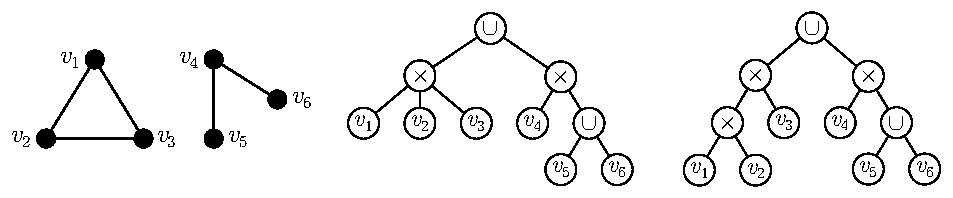
\includegraphics{imagenes/cografos-ejemplo-coarbol.pdf}
    \caption{Ejemplo de un cografo, su coárbol correspondiente, y la
    representación estrictamente binaria del mismo.}
    \label{fig:cografos:ejemplo-coarbol}
\end{figure}

\subsection{Resolución algorítmica}
Sean $G_1 = K_{N_1}$ un grafo completo de $N_1$ nodos (que tendrá por lo tanto
$M_1 = \frac{N_1 \times (N_1 - 1)}{2}$ aristas), y $G_2$ un cografo con $N_2$
nodos y $M_2$ aristas. A la hora de resolver el problema de encontrar el \acr
{MCS} entre $G_1$ y $G_2$, pueden distinguirse estos dos casos:
\begin{enumerate}
    \item $N_1 \geq N_2$. Dado que $G_1$ es un grafo completo, todo
    subgrafo que tenga $N_1$ o menos aristas, y en particular $G_2$,
    es isomorfo a algún subgrafo de $G_1$. Como, trivialmente, $G_2$ es
    isomorfo a sí mismo, basta tomar $G_2$ como solución del problema.
    \item $N_1 < N_2$. En este caso, sea $H$ un grafo isomorfo a algún
    subgrafo de $G_2$; $H$ resultará isomorfo a algún subgrafo de $G_1$ si
    y solo si su cantidad de nodos es menor o igual que $N_1$. Si $H$ tiene
    menos de $N_1$ nodos, puede extenderse a algún grafo $\tilde{H} \supseteq
    H$ que tenga $N_1$ nodos y también sea isomorfo a un subgrafo de $G_2$.
    Es directo que $\tilde{H}$ resulta isomorfo a algún subgrafo de $G_1$ y
    que su cantidad de aristas es mayor o igual que la de $H$. Entonces, si
    $H$ era solución óptima de \acr{MCS}, claramente $\tilde{H}$ también lo
    es. De esto se sigue que para resolver este caso del problema, basta con
    tomar un subgrafo de $G_2$ que tenga exactamente $N_1$ nodos y maximice la
    cantidad de aristas.
\end{enumerate}

Dado que la resolución del primer caso es trivial, durante el resto de esta
sección se asumirá que $N_1 < N_2$. Se llamará $K = N_1$, $G = G_2$, $N = N_2$
y $M = M_2$, y se explicará la solución planteada al problema de encontrar un
subgrafo de un cografo $G$ que tenga exactamente $K$ vértices y cantidad de
aristas máxima.

En general, el problema de determinar para un grafo dado el subgrafo con
determinada cantidad de vértices que maximice la cantidad de aristas es
NP-completo, y por lo tanto, no se conoce un algoritmo eficiente para
resolverlo. No obstante, aprovechando la hipótesis de que $G$ es un cografo,
es posible solucionar el problema en tiempo polinomial.

La solución propuesta tiene dos etapas. En primer lugar, se crea el coárbol
binario de $G$, y luego, utilizando la técnica de programación dinámica, se
aprovecha esta representación para obtener el subgrafo buscado.

\subsubsection{Resultados preliminares}
A continuación, se demostrarán una serie de resultados que serán necesarios
para asegurar la correctitud de los algoritmos presentados más adelante.

\subsubsection{Construcción del coárbol}
Para construir el coárbol correspondiente a un cografo dado, se aprovecha la
en cografos de menor tamaño hasta obtener un conjunto de vértices aislados.
El algoritmo admite una sencilla formulación recursiva: si el cografo consiste
en un vértice aislado, el coárbol tendrá un único nodo representando este
vértice. En caso contrario, el cografo será la unión o el \emph{join} de dos
cografos; el coárbol que lo represente tendrá como raíz un nodo etiquetado con
esa operación, del cual colgarán los coárboles correspondientes a los dos
cografos sobre los cuales esta se aplica.

\subsubsection{Búsqueda del subgrafo máximo}
Para encontrar el subgrafo de $G$ con $K < N$ nodos y máxima cantidad de
aristas, se diseñó un algoritmo utilizando la técnica de programación
dinámica. El esquema detrás de la formulación recursiva de este algoritmo es
la siguiente:

\begin{enumerate}
    \item Si $K = 0$, la solución del algoritmo es un grafo sin nodos ni
    aristas.
    \item Si $K > 0$ y $G = K_1$, es decir, un nodo aislado, la solución es
    $K_1$.
    \item Si $G \neq K_1$, entonces existen dos cografos $G_1$ y $G_2$ tales
    que $G = G_1 \times G_2$ o $G = G_1 \cup G_2$. En tal caso, la solución
    $H$ del problema tendrá algunos de sus nodos en $G_1$ y el resto en $G_2$.
    Entonces, según la operación con la que se obtenga $G$ a partir de $G_1$ y
    $G_2$, tenemos que $H = H_1 \times H_2$ o $H = H_1 \cup H_2$, donde
    $H_1$ y $H_2$ son los subgrafos inducidos en $G$ por los nodos de $H$ que
    pertenecen a $G_1$ y a $G_2$, respectivamente.
\end{enumerate}

\[
    \operatorname{MCS}(G, K) = \begin{cases}
        (\varnothing, \varnothing) & \text{si } K = 0 \\
        K_1 & \text{si } G \text{ es un nodo aislado} \\
        \displaystyle \argmax_{H \in S(G, K)}(\#E(H)) & \text{si } G = (G_1
        \cup G_2) \text{ o } G = (G_1 \times G_2) \\
    \end{cases}
\]

donde

\[
    S(G, K) = \begin{cases}
        \lbrace \operatorname{MCS}(G_1, k) \cup \operatorname{MCS}(G_2, K -
        k) \ \vert\ 0 \leq k \leq K \rbrace & \text{si } G = (G_1 \cup G_2) \\
        \lbrace \operatorname{MCS}(G_1, k) \times \operatorname{MCS}(G_2, K -
        k) \ \vert\ 0 \leq k \leq K \rbrace & \text{si } G = (G_1 \times G_2)
    \end{cases}
\]

\begin{algorithm}[H]
    % \caption{Búsqueda del }
    \Input{Un cografo $G = (V, E)$ con $N$ nodos y $M$ aristas, y un natural
        $K < N$.}
    \Output{Un subgrafo $H \subseteq G$ con $K$ nodos que maximice la cantidad
        de aristas.}

    $cotree$ $\gets$ cotree correspondiente a $G$ \;
    $DP$ $\gets$ grilla de dimensiones $(2 \times N - 1) \times K$, donde \;
    cada fila representa a uno de los vértices del coárbol de $G$, y cada \;
    columna,
    \Return{($DP_{N,M}$, $camino$)}
\end{algorithm}


El algoritmo planteado para la búsqueda del máximo subgrafo


\subsection{Detalles implementativos}

\subsection{Complejidad}
Defino $n_1$ la cantiadad de nodos de $g_1$ (cografo) y $m_1$ la cantiadad de aristas, 
$n_2$ la cantidad de nodos del $g_2$ ($K_n$) 

Armar el cotree tiene una complejidad $O(n_1(n_1 + m_1))$ , hacer el DP que calcula la solucion $O(n_1 * (n_2)^2 )$

En total el algoritmo termina teniendo una complejidad de $O(n_1((n_1 + m_1) + (n_2)^2 ))$

\subsection{Experimentación}

    

    Para la solucion del DP se hicieron tres experimentos:

    \begin{enumerate}
        \item Se Varia los nodos del cografo ($n_1$) y se fija el $K_n$ en 100 nodos, se varia la cantidad de aristas del cografo para ver como afecta al solver DP . Se esperan funciones lineales diferriendo en una constante, dependiendo de como este conectado el cografo. Con este experimento se espera probar la dependencia lineal de $n_1$.
        \item Se varia el cografo en $n$, siendo el cografo un $K_n$  y el segundo grafo en $K_{n/2}$. Se espera funcion cubica , con la cual se pretende mostrar la dependecia cuadratica de $n_2$ y confirmar la depencia lineal de $n_1$.
        \item Se varia el cografo en $n$, siendo el cografo un $K_n$  y el segundo grafo en $K_{log(n)}$. Se espera una funcion de la pint $xlog^2(x)$ , con la cual se pretende mostrar la dependecia cuadratica de $n_2$ y confirmar la depencia lineal de $n_1$.
    \end{enumerate}

    Para la creacion del coarbol se hicieron tres experimentos:

    \begin{enumerate}

        \item Se toma la union de $K_1$, con lo cual se fija la cantidad de aristas en $0$ ($m_1$) y se varia la cantidad de nodos del cografo($n_1$). Se espera una funcion cuadratica, con la cual se quiere mostrar la depencia cuadratica de $n_1$.
        \item Se toma la union de $K_3$, cada 3 nuevos nodos hay 3 nuevas aristas , logrando una dependia lineal $m_1 = n_1$. Se espera una funcion cuadratica con una constante más alta que la union de $K_1$. Con lo cual se espera probar parcialmente la influencia de $m_1$ y confirmar la dependecia cuadratica de $n_1$
        \item Se toma un $K_n$ , con lo cual se tiene una dependencia cuadratica $m_1 = n_1(n_1 - 1)$. Se espera una funcion cuadratica, con la cual se pretende mostrar la influencia de $m_2$.

    \end{enumerate}


    Se experimentó con la creacion del cotree y con la solucion del DP por separado para 
     tener un mayor control de las variables.

 
   \subsubsection{ Experimentos con el solver DP}


    
    \begin{figure}[H]
        \centering
        \begin{tikzpicture}
            \begin{axis}[
                    title={},
                    xlabel={Se Varia los nodos del cografo ($n_1$) y se fija el $K_n$ en 100 nodos.},
                    ylabel={Tiempo de ejecución (nanosegundos)},
                    scaled x ticks=false,
                    scaled y ticks=false,
                    enlargelimits=0.05,
                    width=0.5\textwidth,
                    height=0.5\textwidth,
                    legend pos=north west,
                    legend cell align=left,
                    xmin=100
                ]
                \addplot[color=black] table[x index=0,y index=1]{../exp/ej3/cograph_kn_dp};
                \addplot[color=blue] table[x index=0,y index=1]{../exp/ej3/cograph_k1_union_dp};
                \addplot[color=violet] table[x index=0,y index=1]{../exp/ej3/cograph_k10_union_dp};

                \addplot[color=red] table[x index=0, y expr={ 500000 * (x) }]{../exp/ej3/cograph_kn_dp};
                \legend{$T_{k_n}$,$T_{k_1}$,$T_{k_{10}}$,$ C * x $}
            \end{axis}
        \end{tikzpicture}
        \caption{Se ejecuto la resolucion del DP. como $n_2 = 100$ nos queda una complejidad $O(n1* 100^2)$ = $O(n1)$ }
        \label{fig:exp3:var-nym-base}
    \end{figure}

    Se puede ver que la constante depende del la familia del grafo , ya que $T_{k_n}$ y $T_{k_1}$ tiene una constante muy parecida , ya que uno es el complemento del otro. Queda ver con diversas familias de cografos para ver como afecta al la creacion de coarboles.Se puede esperar mientras más balanceado sea el coarbol más grande sera la constante, ya que en cada paso tendria que probar hijos izquierdos por hijos derechos en el DP.

    

     \begin{figure}[H]
        \centering
        \begin{tikzpicture}
            \begin{axis}[
                    title={},
                    xlabel={Se Varia los nodos del cografo ($n_1$) y se fija el $K_n$ en 100 nodos.},
                    ylabel={Tiempo de ejecución (nanosegundos)},
                    scaled x ticks=false,
                    scaled y ticks=false,
                    enlargelimits=0.05,
                    width=0.5\textwidth,
                    height=0.5\textwidth,
                    legend pos=north west,
                    legend cell align=left,
                    xmin=100
                ];
                \addplot[color=black] table[x index=0,y expr={\thisrowno{1}/(x)} ]{../exp/ej3/cograph_kn_dp};
                \addplot[color=blue] table[x index=0,y expr={\thisrowno{1}/(x)} ]{../exp/ej3/cograph_k1_union_dp};
                \addplot[color=violet] table[x index=0,y expr={\thisrowno{1}/(x)} ]{../exp/ej3/cograph_k10_union_dp};
                \addplot[color=red] table[x index=0, y expr={ 500000 }]{../exp/ej3/cograph_kn_dp};
                \legend{$T_{k_n}$,$T_{k_1}$,$T_{k_{10}}$,$ C * x $}
            \end{axis}
        \end{tikzpicture}
        \caption{Se divide por $n_1$, para mostrar que $C =  500000$ lo acota.}
        \label{fig:exp3:var-nym-base}
    \end{figure}


    


    \begin{figure}[H]
        \centering
        \begin{tikzpicture}
            \begin{axis}[
                    title={},
                    xlabel={Se varia los nodos del cografo, siendo  un $K_n$  y el segundo grafo tiene le mitad de nodos.},
                    ylabel={Tiempo de ejecución (nanosegundos)},
                    scaled x ticks=false,
                    scaled y ticks=false,
                    enlargelimits=0.05,
                    width=0.5\textwidth,
                    height=0.5\textwidth,
                    legend pos=north west,
                    legend cell align=left,
                    xmin=0
                ]
                \addplot[color=black] table[x index=0,y index=1]{../exp/ej3/cograph_kn_and_k_n_div_2_dp};
                \addplot[color=red] table[x index=0, y expr={ 10 * (x*x*x) }]{../exp/ej3/cograph_kn_and_k_n_div_2_dp};
                \legend{$T_{k_n}$,$ C * x^3 $}
            \end{axis}
        \end{tikzpicture}
        \caption{Se ejecuto la resolucion del DP. como $n_2 = n_1/2$ nos queda una complejidad $O(n_1* (n_1/2)^2)$ = $O(n_1^3)$}
        \label{fig:exp3:var-nym-base}
    \end{figure}

    \begin{figure}[H]
        \centering
        \begin{tikzpicture}
            \begin{axis}[
                    title={},
                    xlabel={Se varia los nodos del cografo, siendo  un $K_n$  y el segundo grafo tiene le mitad de nodos.},
                    ylabel={Tiempo de ejecución (nanosegundos)},
                    scaled x ticks=false,
                    scaled y ticks=false,
                    enlargelimits=0.05,
                    width=0.5\textwidth,
                    height=0.5\textwidth,
                    legend pos=north west,
                    legend cell align=left,
                    xmin=0
                ]
                \addplot[color=black] table[x index=0,y expr={\thisrowno{1}/(x*x*x)}]{../exp/ej3/cograph_kn_and_k_n_div_2_dp};
                \addplot[color=red] table[x index=0, y expr={ 10}]{../exp/ej3/cograph_kn_and_k_n_div_2_dp};
                \legend{$T_{k_{n/2}}$,$ C $}
            \end{axis}
        \end{tikzpicture}
        \caption{Se divide por $n_1^2$, para mostrar, que $C =  10$ lo acota.  }
        \label{fig:exp3:var-nym-base}
    \end{figure}

    


    
    \begin{figure}[H]
        \centering
        \begin{tikzpicture}
            \begin{axis}[
                    title={},
                    xlabel={Se varia el cografo en $n$, siendo el cografo un $K_n$  y el segundo grafo en $K_{ln(n)}$.},
                    ylabel={Tiempo de ejecución (nanosegundos)},
                    scaled x ticks=false,
                    scaled y ticks=false,
                    enlargelimits=0.05,
                    width=0.5\textwidth,
                    height=0.5\textwidth,
                    legend pos=north west,
                    legend cell align=left,
                    xmin=0
                ]
                \addplot[color=black] table[x index=0,y index=1]{../exp/ej3/cograph_kn_and_k_log_n_dp};
                \addplot[color=red] table[x index=0, y expr={ 135 * x * ln(x) * ln(x) }]{../exp/ej3/cograph_kn_and_k_log_n_dp};
       
                \legend{$T_{k_{ln(n)}}$,$ C * x * ln^2(x) $}
            \end{axis}
        \end{tikzpicture}
        \caption{Se ejecuto la resolucion del DP. como $n_2 = ln(n_1)$ nos queda una complejidad $O(n_1 * ln^2(n_1))$}
        \label{fig:exp3:var-nym-base}
    \end{figure}


    \begin{figure}[H]
        \centering
        \begin{tikzpicture}
            \begin{axis}[
                    title={},
                    xlabel={Se varia el cografo en $n$, siendo el cografo un $K_n$  y el segundo grafo en $K_{ln(n)}$.},
                    ylabel={Tiempo de ejecución (nanosegundos)},
                    scaled x ticks=false,
                    scaled y ticks=false,
                    enlargelimits=0.05,
                    width=0.5\textwidth,
                    height=0.5\textwidth,
                    legend pos=north west,
                    legend cell align=left,
                    xmin=0
                ]
                
                \addplot[color=black] table[x index=0,y expr={\thisrowno{1}/(x)}]{../exp/ej3/cograph_kn_and_k_log_n_dp};
                \addplot[color=red] table[x index=0, y expr={ 135 * ln(x) * ln(x)  }]{../exp/ej3/cograph_kn_and_k_log_n_dp};
                \legend{$T_{k_{ln(n)}}$,$ C * ln^2(x) $}
            \end{axis}
        \end{tikzpicture}
        \caption{Se divide por $n_1$, para mostrar que $C * ln^2(x)$ lo acota. }
        \label{fig:exp3:var-nym-base}
    \end{figure}

    \begin{figure}[H]
        \centering
        \begin{tikzpicture}
            \begin{axis}[
                    title={},
                    xlabel={Se varia el cografo en $n$, siendo el cografo un $K_n$  y el segundo grafo en $K_{ln(n)}$.},
                    ylabel={Tiempo de ejecución (nanosegundos)},
                    scaled x ticks=false,
                    scaled y ticks=false,
                    enlargelimits=0.05,
                    width=0.5\textwidth,
                    height=0.5\textwidth,
                    legend pos=north west,
                    legend cell align=left,
                    xmin=0
                ]
                
                \addplot[color=black] table[x index=0,y expr={\thisrowno{1}/(x * ln(x) * ln(x)) }]{../exp/ej3/cograph_kn_and_k_log_n_dp};
                \addplot[color=red] table[x index=0, y expr={ 135 }]{../exp/ej3/cograph_kn_and_k_log_n_dp};
                \legend{$T_{k_{ln(n)}}$,$ C $}
            \end{axis}
        \end{tikzpicture}
        \caption{Se divide por $x * ln^2(x)$, para mostrar, que $C =  135$ lo acota.}
        \label{fig:exp3:var-nym-base}
    \end{figure}









    \subsubsection{Experimentos con la creacion del coarbol}




    \begin{figure}[H]
        \centering
        \begin{tikzpicture}
            \begin{axis}[
                    title={},
                    xlabel={Se fija la cantidad de aristas en $0$ ($m_1$) y se varia la cantidad de nodos del cografo($n_1$).},
                    ylabel={Tiempo de ejecución (nanosegundos)},
                    scaled x ticks=false,
                    scaled y ticks=false,
                    enlargelimits=0.05,
                    width=0.5\textwidth,
                    height=0.5\textwidth,
                    legend pos=north west,
                    legend cell align=left,
                    xmin=0
                ]
                \addplot[color=black] table[x index=0,y index=1]{../exp/ej3/cograph_k1_union_create_cotree};
                \addplot[color=red] table[x index=0, y expr={ 12 * (x*x) }]{../exp/ej3/cograph_k1_union_create_cotree};
                \legend{$T_{K_1}$,$ C * x^2 $}
            \end{axis}
        \end{tikzpicture}
        \caption{Se ejecuta la creacion del coarbol. como $m_2 = 0$ nos queda una complejidad $O(n_1(n_1 + 0))$ = $O(n_1^2$}
        \label{fig:exp3:var-nym-base}
    \end{figure}


       \begin{figure}[H]
        \centering
        \begin{tikzpicture}
            \begin{axis}[
                    title={},
                    xlabel={Se fija la cantidad de aristas en $0$ ($m_1$) y se varia la cantidad de nodos del cografo($n_1$).},
                    ylabel={Tiempo de ejecución (nanosegundos)},
                    scaled x ticks=false,
                    scaled y ticks=false,
                    enlargelimits=0.05,
                    width=0.5\textwidth,
                    height=0.5\textwidth,
                    legend pos=north west,
                    legend cell align=left,
                    xmin=0,
                    ymax= 50
                ]
                \addplot[color=black] table[x index=0,y expr={\thisrowno{1}/(x*x)}]{../exp/ej3/cograph_k1_union_create_cotree};
                \addplot[color=red] table[x index=0, y expr={ 12 }]{../exp/ej3/cograph_k1_union_create_cotree};
                \legend{$T_{K_1}$,$ C $}
            \end{axis}
        \end{tikzpicture}
        \caption{Se divide por $n_1^2$, para mostrar, que $C =  12$ lo acota.}
        \label{fig:exp3:var-nym-base}
    \end{figure}


    \begin{figure}[H]
        \centering
        \begin{tikzpicture}
            \begin{axis}[
                    title={},
                    xlabel={Se toma la uniones de $K_3$},
                    ylabel={Tiempo de ejecución (nanosegundos)},
                    scaled x ticks=false,
                    scaled y ticks=false,
                    enlargelimits=0.05,
                    width=0.5\textwidth,
                    height=0.5\textwidth,
                    legend pos=north west,
                    legend cell align=left,
                    xmin=0
                ]
                \addplot[color=black] table[x index=0,y index=1]{../exp/ej3/cograph_k3_union_create_cotree};
                \addplot[color=red] table[x index=0, y expr={  140 * (x*x) }]{../exp/ej3/cograph_k3_union_create_cotree};
                \legend{$T_{K_3}$,$ C * x^2 $}
            \end{axis}
        \end{tikzpicture}
        \caption{Se ejecuta la creación del cotree. Como $m_1 = n_1$ nos queda una complejidad $O(n_1(n_1 + n_1))$ = $O(n_1^2)$}
        \label{fig:exp3:var-nym-base}
    \end{figure}

      \begin{figure}[H]
        \centering
        \begin{tikzpicture}
            \begin{axis}[
                    title={},
                    xlabel={Se toma la uniones de $K_3$.},
                    ylabel={Tiempo de ejecución (nanosegundos)},
                    scaled x ticks=false,
                    scaled y ticks=false,
                    enlargelimits=0.05,
                    width=0.5\textwidth,
                    height=0.5\textwidth,
                    legend pos=north west,
                    legend cell align=left,
                    xmin=0,
                    ymax= 200
                ]
                \addplot[color=black] table[x index=0,y expr={\thisrowno{1}/(x*x)}]{../exp/ej3/cograph_k3_union_create_cotree};
                \addplot[color=red] table[x index=0, y expr={140}]{../exp/ej3/cograph_k3_union_create_cotree};
                \legend{$T_{K_3}$,$ C $}
            \end{axis}
        \end{tikzpicture}
        \caption{Se divide por $n_1^2$, para mostrar, que $C =  140$ lo acota.}
        \label{fig:exp3:var-nym-base}
    \end{figure}





    \begin{figure}[H]
        \centering
        \begin{tikzpicture}
            \begin{axis}[
                    title={},
                    xlabel={Se toma un $K_{n_1}$},
                    ylabel={Tiempo de ejecución (nanosegundos)},
                    scaled x ticks=false,
                    scaled y ticks=false,
                    enlargelimits=0.05,
                    width=0.5\textwidth,
                    height=0.5\textwidth,
                    legend pos=north west,
                    legend cell align=left,
                    xmin=0
                ]
                \addplot[color=black] table[x index=0,y index=1]{../exp/ej3/cograph_kn_create_cotree};
                \addplot[color=red] table[x index=0, y expr={ 17 * (x*x*x) }]{../exp/ej3/cograph_kn_create_cotree};
                \legend{$T_{k_{n_1}}$,$ C * x^3 $}
            \end{axis}
        \end{tikzpicture}
        \caption{Se ejecuta la creación del cotree. Como $m_1 = n_1(n_1 - 1) = n_1^2 -n_1 $ nos queda una complejidad  $O(n_1(n_1 + n_1^2 -n_1))$ = $O(n_1^3)$ }
        \label{fig:exp3:var-nym-base}
    \end{figure}

     \begin{figure}[H]
        \centering
        \begin{tikzpicture}
            \begin{axis}[
                    title={},
                    xlabel={Se toma un $K_{n_1}$},
                    ylabel={Tiempo de ejecución (nanosegundos)},
                    scaled x ticks=false,
                    scaled y ticks=false,
                    enlargelimits=0.05,
                    width=0.5\textwidth,
                    height=0.5\textwidth,
                    legend pos=north west,
                    legend cell align=left,
                    xmin=0,
                    ymax= 50
                ]
                \addplot[color=black] table[x index=0,y expr={\thisrowno{1}/(x*x*x)}]{../exp/ej3/cograph_kn_create_cotree};
                \addplot[color=red] table[x index=0, y expr={ 17 }]{../exp/ej3/cograph_kn_create_cotree};
                \legend{$T_{k_{n_1}}$,$C$}
            \end{axis}
        \end{tikzpicture}
        \caption{Se divide por $n_1^3$, para mostrar, que $C =  17$ lo acota.}
        \label{fig:exp3:var-nym-base}
    \end{figure}

    \subsubsection{Concluciones}
    
    Se puede concluir que armar el cotree tiene una complejidad $O(n_1(n_1 + m_1))$ y resolver el DP $O(n_1 * (n_2)^2 )$.
    Como el agoritmo, arma el cotree y despues resuelve el DP , nos queda una complejidad de $O(n_1(n_1 + m_1)) + O(n_1 * (n_2)^2 )$ = $O(n_1((n_1 + m_1) + (n_2)^2 ))$.





   
















\newpage
\section{Heurística golosa}

% Desgraciadamente, el problema es tan difícil que ni Marty ni el Doc conocen
% una manera de resolverlo en tiempo polinomial para el caso general. Para no
% quedarse con las manos vacías, Marty les pide diseñar e implementar una
% heurística constructiva golosa para MCS y desarrollar los siguientes puntos
% para conocer la calidad de las soluciones que le proveerán:
% a) Explicar detalladamente el algoritmo implementado.
% b) Calcular el orden de complejidad temporal de peor caso del algoritmo.
% c) Describir instancias de MCS para las cuales la heurística no proporciona
%    una solución óptima. Indicar qué tan mala puede ser la solución obtenida
%    respecto de la solución óptima.
% d) Realizar una experimentación que permita observar la performance del
%    algoritmo en términos de tiempo de ejecución en función del tamaño de
%    entrada.

\subsection{Introducción}

Dado que la complejidad del algoritmo exacto resulta prohibitiva en la práctica,
se pedía desarrollar una heurística golosa que resolviera el problema en tiempo
polinomial. Para esto fue necesario plantear algoritmos que a cuestas de la
calidad final de la solución permitieran mejorar sustancialmente la complejidad.

Pensar heurísticas tiene el desafío de que las mismas suelen tener un factor
importante de intuición sobre por qué podrían llegar a funcionar mejor o peor y
no una justificación formal. Esto tiene como consecuencia que resulta
difícil decidir qué criterio utilizar puesto que siempre es posible
encontrar instancias para las cuales el mismo sea tan malo como uno
quiera.

El criterio seleccionado fue el grado de los nodos. La motivación detrás de esta
decisión fue la idea de que tomando los vértices de mayor grado en cada grafo,
uno aumenta la posibilidad de que tengan vecinos en común, permitiendo así mapear
sus respectivas aristas en el subgrafo común.

\subsection{Experimentación}

\pgfplotstableread[header=false]{../exp/ej4/known_sol_greedy_exp}\knowngreedy
\pgfplotstableread[header=false]{../exp/optimal_solutions}\optimalsolutions

\pgfplotstableset{
	create on use/sol/.style={copy column from table={\optimalsolutions}{[index] 1}}
}

\pgfplotstabletypeset[
	every head row/.style={
		after row=\hline
	},
	columns={0, sol, 1, 3, 4},
	columns/0/.style={
		column name=\textsc{Instancia},
		column type={l},
		string replace*={_}{\_},
		string type,
		assign cell content/.code={
			\pgfkeyssetvalue{/pgfplots/table/@cell content}{\texttt{##1}}
		}
	},
	columns/sol/.style={
		column name=$\#E(MCS)$,
		int detect
	},
	columns/1/.style={
		column name=$\#E(H)$,
		int detect
	},
	columns/3/.style={
		column name=$T_{\mu}$,
	},
	columns/4/.style={
		column name=$T_{\sigma}$,
	}
]\knowngreedy


\newpage
\section{Heurística de búsqueda local}

% Obviamente, el Doc está en desacuerdo y dice que la heurística golosa no es
% la mejor idea. Para justificar su postura les pide diseñar e implementar una
% heurística de búsqueda local para MCS, y desarrollar los siguientes puntos
% para, de una buena vez, convencer a Marty:
% a) Explicar detalladamente el algoritmo implementado. Plantear al menos dos
%    vecindades distintas para la búsqueda.
% b) Calcular el orden de complejidad temporal de peor caso de una iteración
%    del algoritmo de búsqueda local (para las vecindades planteadas). Si es
%    posible, dar una cota superior para la cantidad de iteraciones de la
%    heurística.
% c) Realizar una experimentación que permita observar la performance del
%    algoritmo comparando los tiempos de ejecución y la calidad de las
%    soluciones obtenidas, en función de las vecindades utilizadas y elegir,
%    si es posible, la configuración que mejores resultados provea para el
%    grupo de instancias utilizado.

\subsection{Introducción}
Este ejercicio consiste en la implementación de una heurística de búsqueda
local para el problema de \acr{MCS}, que sea capaz de iterar sobre una
solución dada y mejorarla en búsqueda de óptimos locales.

Al igual que en el ejercicio anterior, asumiremos sin pérdida de generalidad
que los grafos $G_1$ y $G_2$ para los que quiere resolverse el problema son
tales que $N_1 \leq N_2$, siendo $N_1$ y $N_2$ sus cantidades de nodos
respectivas.

\subsection{Vecindades planteadas}

El principal elemento a definir a la hora de plantear una heurística de
búsqueda local es qué soluciones se considerarán vecinas. Es decir, es
necesario plantear una \emph{relación de vecindad} entre el espacio de
soluciones del problema. Para esto, será útil adoptar de nuevo el enfoque
de ver a una solución de \acr{MCS} como un mapeo $s : V(G_1) \to V(G_2)$.
De esta forma, se define el espacio de soluciones posibles del problema como
\[ S = \lbrace s : V(G_1) \to V(G_2) \ \vert\ s \text{ es inyectiva}
\rbrace \]
y se plantean dos alternativas para definir una relación simétrica $N
\subseteq S \times S$.
Luego, dada una solución del problema $s \in S$, la heurística
explorará todas las soluciones vecinas de $s$, es decir, aquellas que se
relacionen con $s$ a través de $N$.

Una característica que se tuvo en cuenta a la hora de definir las vecindades
fue que cualquier solución fuera alcanzable desde cualquier otra, moviéndose
sucesivas veces entre soluciones vecinas.

A continuación se describen las dos vecindades planteadas, junto con el
pseudocódigo del algoritmo que itera sobre cada una de ellas y selecciona,
dada una solución cualquiera, la mejor entre sus soluciones vecinas. También
se calcula, en cada caso, una cota teórica para la complejidad de dicho
algoritmo. Para esto se tienen en cuenta las estructuras utilizadas al
implementarlo; muchas de las operaciones que se consideran $\ord(1)$ lo son en
realidad al considerar el costo amortizado, dado que varios de los mapeos
necesarios se implementan mediante tablas de \emph{hash}.

\subsubsection{Vecindad I}
Dos soluciones $s, s' \in S$ se consideran vecinas en la vecindad I
si $s'$ es el resultado de modificar el mapeo de exactamente uno de los nodos
de $G_1$ en $s$, asignándole un nodo de $G_2$ que esté libre en $s$. Es
decir, $(s, s') \in N_1$ si y solo si
\begin{itemize}
    \item $(\exists \ v \in G_1)\ s(v) \neq s'(v)$, y
    \item $(\forall \ w \in G_1)\ w \neq v \Rightarrow s(w) = s'(w)$.
\end{itemize}

Es importante notar que esta vecindad no está bien definida, y por lo tanto no
puede aplicarse, si $\#V(G_1) = \#V (G_2)$.

\begin{figure}[htbp]
    \centering
    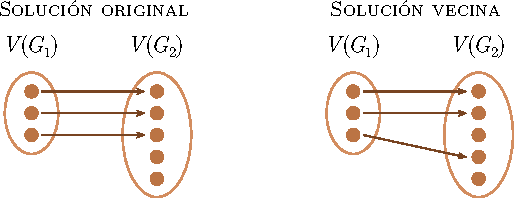
\includegraphics{imagenes/ex5_vecindad1.pdf}
    \caption{Ejemplo de soluciones vecinas que es posible obtener mediante la
    vecindad I.}
    \label{fig:ej5:vecindad1}
\end{figure}

\subheading{Pseudocódigo de una iteración}

\begin{algorithm}[H]
    \SetAlgoVlined
    \caption{Iteración de la vecindad I}
    \Input{Dos grafos $G_1$ y $G_2$, con $\#V(G_1) < \#V(G_2)$, y un tercer
    grafo \textit{solución}, cuyos nodos son pares de $V(G_1) \times V(G_2)$,
    representando la solución a \acr{MCS} que se pretende mejorar. Este último
    grafo será modificado por el algoritmo.}
    \Output{Un valor de verdad indicando si se pudo mejorar la solución.}
    \textit{hay\_mejora} $\gets$ \textsf{falso} \;
    \textit{mejor\_diferencia\_aristas} $\gets$ 0 \;

    \ForEach{vértice $(v, w)$ de \textit{solución}} {
        \ForEach{vértice $w'$ de $G_2$ que no esté en el mapeo} {
            \textit{cant\_aristas\_perdidas} $\gets$ grado de $(v, w)$ en \textit{solución} \;
            \textit{aristas\_nuevas} $\gets$ vector vacío \;
            \ForEach {vecino $\tilde{w}$ de $w_2$ en $G_2$} {
                \If{$\tilde{w}$ está en el mapeo} {
                    $\tilde{v}$ $\gets$ nodo de $G_1$ al que está mapeado $\tilde{w}$ \;
                    \If{$\tilde{v}$ es vecino de $v$ en $G_1$} {
                        agregar $(\tilde{v}, \tilde{w})$ a \textit{aristas\_nuevas} \;
                    }
                }
            }
            \textit{diferencia\_aristas} $\gets$ $\vert$\textit{aristas\_nuevas}$\vert$
                $-$ \textit{cant\_aristas\_perdidas} \;
            \If{\textit{diferencia\_aristas} $>$ \textit{mejor\_diferencia\_aristas}} {
                \textit{hay\_mejora} $\gets$ \textsf{verdadero} \;
                \textit{mejor\_diferencia\_aristas} $\gets$ \textit{diferencia\_aristas} \;
                \textit{mejor\_para\_eliminar} $\gets$ $(v, w)$ \;
                \textit{mejor\_para\_agregar} $\gets$ $(v, w')$ \;
                \textit{mejor\_aristas\_nuevas} $\gets$ \textit{aristas\_nuevas} \;
            }
        }
    }
    \eIf{\textit{hay\_mejora}} {
        eliminar el nodo \textit{mejor\_para\_eliminar} de \textit{solución} \;
        agregar el nodo \textit{mejor\_para\_agregar} a \textit{solución} \;
        \ForEach{par $(\tilde{v}, \tilde{w})$ en \textit{mejor\_aristas\_nuevas}} {
            agregar en \textit{solución} una arista entre
                \textit{mejor\_para\_agregar} y $(\tilde{v}, \tilde{w})$ \;
        }
        \Return{\textsf{verdadero}}
    } {
        \Return{\textsf{falso}}
    }
\end{algorithm}

\subheading{Complejidad temporal}

Cada iteración del algoritmo recorre la vecindad completa de la solución que
se busca mejorar; para esto se utilizan dos ciclos anidados. El primero de
ellos recorre todos los nodos de la solución, es decir, realiza $N_1$
iteraciones. El ciclo interior recorre el conjunto $W_U \subseteq G_2$ de los
nodos de $G_2$ que no forman parte del mapeo, que tiene $N_2 - N_1$ elementos.
Dentro de este ciclo, además de realizarse operaciones con un costo constante,
se itera a su vez, para cada nodo $w \in W_U$, sobre el conjunto de sus
vecinos, cuyo cardinal es $\deg(w)$. Para cada uno de estos vecinos se
verifica si pertenece al mapeo y, en caso afirmativo, debe decidirse si son
adyacentes en $G_1$ los nodos mapeados a $w$ y su vecino en cuestión. Esto
último tiene complejidad $\ord(\deg(v))$, siendo $v$ el nodo de $G_1$
mapeado a $w$, que puede acotarse por $\ord(N_1)$. De todo lo anterior se
concluye que la complejidad del primer ciclo es:

\begin{align*}
\ord\left( N_1 \times \left( \sum_{w \in W_U} \left(1 + \deg(w) \times N_1
\right) \right) \right)
&= \ord \left( N_1 \times \left( (N_2 - N_1) + N_1 \times \sum_{W \in W_U}
\deg(w) \right) \right) \\
&= \ord \left( N_1 \times \left( (N_2 - N_1) + N_1 \times \sum_{w \in V(G_2)}
\deg(w) \right) \right) \\
&= \ord \left( N_1 \times \left( (N_2 - N_1) + N_1 \times M_2 \right) \right) \\
&= \ord \left( N_1 \times (N_2 - N_1) + N_1^2 \times M_2 \right)
\end{align*}

En la segunda parte del algoritmo, si se encontró alguna mejora a la solución,
deben modificarse las estructuras que se utilizan para almacenar la misma. En
primer lugar se elimina un nodo de la solución; el costo de esta operación es
el grado de dicho nodo. Dado que todas las aristas adyacentes a un nodo de la
solución deben corresponderse con aristas en $G_1$, el grado máximo de un nodo
en la solución está acotado por el grado máximo de un nodo de $G_1$, que es
$N_1 - 1$. Luego se agrega a la solución un nuevo nodo; esto tiene un costo de
orden $\ord(N_2 - N_1)$, ya que debe eliminarse el vértice de un vector que
almacena los nodos que no pertenecen al mapeo. Por último se incorporan, cada
una con un costo constante, todas las aristas correspondientes al nuevo nodo,
cuya cantidad está igualmente acotada por $N_1 - 1$.

De esta forma, la segunda parte de la iteración tiene un costo de $\ord(N_2 -
N_1) + \ord(N_1) = \ord (N_1 + N_2)$, que resulta absorbido por el costo de
recorrer la vecindad, obteniendo una complejidad total para cada iteración de
\[ \ord \left( N_1 \times (N_2 - N_1) + N_1^2 \times M_2 \right) \]

\subsubsection{Vecindad II}
Dos soluciones $s, s' \in S$ se consideran vecinas en la vecindad II
si $s'$ es el resultado de aplicar sobre $s$ alguno de estos cambios:
\begin{itemize}
    \item \textsc{Permutación:} permutar los mapeos de dos nodos de $G_1$, de
    forma tal que $s'(v_1) = s(v_2)$ y $s'(v_2) = s(v_1)$. Formalmente,
    \begin{itemize}
        \item $(\exists \ v_1, v_2 \in G_1)\ s'(v_1) = s(v_2)$ y $s'(v_2) = s
        (v_1)$, y
        \item $(\forall \ w \in G_1)\ w \neq v_1$ y $w \neq v_2
        \Rightarrow s(w) = s'(w)$.
    \end{itemize}
    \item \textsc{Intercambio:} la misma operación que define la vecindad
    I, es decir, modificar el mapeo de exactamente uno de los nodos
    de $G_1$, asignándole un nodo de $G_2$ que esté libre en $s$. Formalmente,
    \begin{itemize}
        \item $(\exists \ v \in G_1)\ s(v) \neq s'(v)$, y
        \item $(\forall \ w \in G_1)\ w \neq v \Rightarrow s(w) = s'(w)$.
    \end{itemize}
\end{itemize}

La vecindad II no tiene problemas de definición en el caso de que $\#V(G_1)
= \#V (G_2)$.

\begin{figure}[htbp]
    \centering
    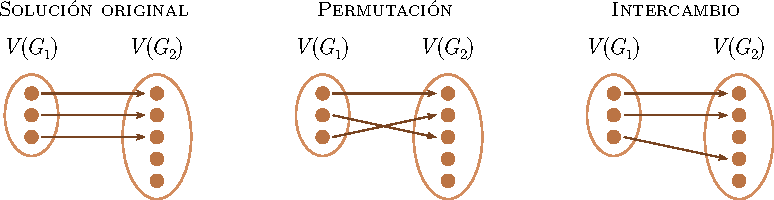
\includegraphics{imagenes/ex5_vecindad2.pdf}
    \caption{Soluciones vecinas que es posible obtener mediante la vecindad
    II.}
    \label{fig:ej5:vecindad2}
\end{figure}

Cabe destacar que la vecindad I está contenida en la vecindad II,
siendo esta última considerablemente más grande. Desde un punto de vista
computacional, esto tiene como desventaja inmediata un mayor costo a la hora
de recorrer y explorar la vecindad, pero corre con la ventaja de que resulta
posible pasar de una solución dada a cualquier otra en una cantidad de
iteraciones menor (se puede decir que $N_2$ es una vecindad más
\emph{densamente conectada} que I).

\subheading{Pseudocódigo de una iteración}

\begin{algorithm}[H]
    \SetAlgoVlined
    \caption{Iteración de la vecindad II}
    \Input{Dos grafos $G_1$ y $G_2$, con $\#V(G_1) < \#V(G_2)$, y un tercer
    grafo \textit{solución}, cuyos nodos son pares de $V(G_1) \times V(G_2)$,
    representando la solución a \acr{MCS} que se pretende mejorar. Este último
    grafo será modificado por el algoritmo.}
    \Output{Un valor de verdad indicando si se pudo mejorar la solución.}
    \textit{hay\_mejora} $\gets$ \textsf{falso} \;
    \textit{mejor\_diferencia\_aristas} $\gets$ 0 \;

    \ForEach{vértice $w_1$ de $G_2$} {
        \ForEach{vértice $w_2$ de $G_2$} {
            \textit{diferencia\_aristas} $\gets$ $0$ \;
            \uIf{$w_1$ y $w_2$ están en el mapeo} {
                (Código extraido como Algoritmo \ref{alg:ej5:vec2:permutacion})
            }
            \ElseIf{$w_1$ está en el mapeo o $w_2$ está en el mapeo} {
                (Código extraido como Algoritmo \ref{alg:ej5:vec2:intercambio})
            }
            \If{\textit{diferencia\_aristas} $>$ \textit{mejor\_diferencia\_aristas}} {
                \textit{hay\_mejora} $\gets$ \textsf{verdadero} \;
                \textit{mejor\_diferencia\_aristas} $\gets$ \textit{diferencia\_aristas} \;
                \textit{mejor\_acción} $\gets$ \textit{acción} \;
                \textit{mejor\_1} $\gets$ $(v_1, w_1)$ \;
                \textit{mejor\_2} $\gets$ $(v_2, w_2)$ \;
                \textit{mejor\_aristas\_nuevas\_1} $\gets$ \textit{aristas\_nuevas\_1} \;
                \textit{mejor\_aristas\_nuevas\_2} $\gets$ \textit{aristas\_nuevas\_2} \;
            }
        }
    }
    \eIf{\textit{hay\_mejora}} {
        \uIf{\textit{mejor\_acción} $=$ \textsf{permutación}} {
            eliminar los nodos \textit{mejor\_1} y \textit{mejor\_2} de \textit{solución} \;
            \textit{nuevo\_1} $\gets$ (\textit{mejor\_1}.primero, \textit{mejor\_2}.segundo) \;
            \textit{nuevo\_2} $\gets$ (\textit{mejor\_2}.primero, \textit{mejor\_1}.segundo) \;
            agregar los nodos \textit{nuevo\_1} y \textit{nuevo\_2} a \textit{solución}\;
            \If {\textit{mejor\_1} y \textit{mejor\_2} eran adyacentes en \textit{solución}} {
                agregar en \textit{solución} una arista entre \textit{mejor\_1} y \textit{mejor\_2} \;
            }
            \ForEach{par $(\tilde{v}, \tilde{w})$ en \textit{mejor\_aristas\_nuevas\_1}} {
                agregar en \textit{solución} una arista entre
                    \textit{mejor\_1} y $(\tilde{v}, \tilde{w})$ \;
            }
            \ForEach{par $(\tilde{v}, \tilde{w})$ en \textit{mejor\_aristas\_nuevas\_2}} {
                agregar en \textit{solución} una arista entre
                    \textit{mejor\_2} y $(\tilde{v}, \tilde{w})$ \;
            }
        }
        \ElseIf{\textit{mejor\_accion} $=$ \textsf{intercambio}} {
            eliminar el nodo \textit{mejor\_1} de \textit{solución} \;
            agregar el nodo \textit{mejor\_2} a \textit{solución} \;
            \ForEach{par $(\tilde{v}, \tilde{w})$ en \textit{mejor\_aristas\_nuevas\_1}} {
                agregar en \textit{solución} una arista entre
                    \textit{mejor\_1} y $(\tilde{v}, \tilde{w})$ \;
            }
        }
        \Return{\textsf{verdadero}}
    } {
        \Return{\textsf{falso}}
    }
\end{algorithm}
\bigskip

\begin{algorithm}[H]
    \SetAlgoVlined
    \caption{Iteración de la vecindad II (Sección correspondiente a la acción \textsc{Permutación})}
    \label{alg:ej5:vec2:permutacion}
    \textit{acción} $\gets$ \textsf{permutación} \;
    $v_1$ $\gets$ nodo de $G_1$ al que está mapeado $w_1$ \;
    $v_2$ $\gets$ nodo de $G_1$ al que está mapeado $w_2$ \;
    \textit{cant\_aristas\_perdidas} $\gets$ (grado de $(v_1, w_1)$ en \textit{solución}) +
        (grado de $(v_2, w_2)$ en \textit{solución}) \;
    \If{$(v_1, w_1)$ es adyacente a $(v_2, w_2)$ en \textit{solución}} {
        \textit{cant\_aristas\_perdidas} $\gets$ \textit{cant\_aristas\_perdidas} $-$ $2$ \;
    }
    \textit{aristas\_nuevas\_1} $\gets$ vector vacío \;
    \ForEach{vecino $\tilde{w}$ de $w_1$ en $G_2$} {
        \If{$\tilde{w} \neq w_2$ y $\tilde{w}$ está en el mapeo} {
            $\tilde{v}$ $\gets$ nodo de $G_1$ al que está mapeado $\tilde{w}$ \;
            \If{$\tilde{v}$ es vecino de $v_1$ en $G_1$} {
                agregar $(\tilde{v}, \tilde{w})$ a \textit{aristas\_nuevas\_1} \;
            }
        }
    }
    \textit{aristas\_nuevas\_2} $\gets$ vector vacío \;
    \ForEach{vecino $\tilde{w}$ de $w_2$ en $G_2$} {
        \If{$\tilde{w} \neq w_1$ y $\tilde{w}$ está en el mapeo} {
            $\tilde{v}$ $\gets$ nodo de $G_1$ al que está mapeado $\tilde{w}$ \;
            \If{$\tilde{v}$ es vecino de $v_2$ en $G_1$} {
                agregar $(\tilde{v}, \tilde{w})$ a \textit{aristas\_nuevas\_2} \;
            }
        }
    }
    \textit{diferencia\_aristas} $\gets$ $\vert$\textit{aristas\_nuevas\_1}$\vert$ $+$
        $\vert$\textit{aristas\_nuevas\_2}$\vert$ $-$ \textit{cant\_aristas\_perdidas} \;
\end{algorithm}
\bigskip

\begin{algorithm}[H]
    \SetAlgoVlined
    \caption{Iteración de la vecindad II (Sección correspondiente a la acción \textsc{Intercambio})}
    \label{alg:ej5:vec2:intercambio}
    \textit{acción} $\gets$ \textsf{intercambio} \;
    \If{$w_1$ no forma parte del mapeo} {
        llamar $w_1$ a $w_2$ y viceversa (para poder asumir
            que $w_1$ es el nodo que está mapeado) \;
    }
    $v_1$ $\gets$ nodo de $G_1$ al que está mapeado $w_1$ \;
    $v_2$ $\gets$ $v_1$ \;
    \textit{cant\_aristas\_perdidas} $\gets$ grado de $(v_1, w_1)$ en \textit{solución} \;
    \textit{aristas\_nuevas\_1} $\gets$ vector vacío \;
    \ForEach {vecino $\tilde{w}$ de $w_2$ en $G_2$} {
        \If{$\tilde{w}$ está en el mapeo} {
            $\tilde{v}$ $\gets$ nodo de $G_1$ al que está mapeado $\tilde{w}$ \;
            \If{$\tilde{v}$ es vecino de $v_1$ en $G_1$} {
                agregar $(\tilde{v}, \tilde{w})$ a \textit{aristas\_nuevas\_1} \;
            }
        }
    }
    \textit{diferencia\_aristas} $\gets$ $\vert$\textit{aristas\_nuevas}$\vert$
        $-$ \textit{cant\_aristas\_perdidas} \;
\end{algorithm}

\subheading{Complejidad temporal}

Dado que el tamaño de esta vecindad es mayor al de la otra alternativa
planteada, también será más costosa cada iteración que deba explorarla. El
recorrido se hace mediante dos ciclos anidados, cada uno de los cuales se
repite $N_2$ veces. De esta forma se recorren todos los pares posibles de
dos nodos de $G_2$. No obstante, debido a que según el caso el código que se
ejecuta en cada una de estas repeticiones es diferente, se estudiará la
complejidad de cada uno de ellos por separado.

\begin{itemize}
    \item La operación de \emph{permutación} se realiza cuando se
    selecciona un par de nodos distintos $w_1, w_2$ de $W_M \subseteq G_2$,
    siendo $W_M$ el conjunto de los nodos que pertenecen al mapeo (cuyo
    cardinal es $N_1$). Como la cantidad de estos nodos es $N_1$, este tipo de
    iteración se ejecuta $\ord(N_1^2)$ veces. Además de operaciones con costo
    constante, dentro de cada repetición de este proceso se ejecutan dos
    ciclos, uno de los cuales itera sobre los vecinos de $w_1$ ($\deg(w_1)$) y
    el otro, sobre los vecinos de $w_2$ ($\deg(w_2)$). Para cada uno de ellos
    se chequea su adyacencia en $G_1$ con los nodos mapeados a $w_1$ y $w_2$,
    respectivamente, lo cual tiene un costo acotable por $\ord(N_1)$.

    Es importante notar que el primer ciclo se ejecutará exactamente $N_1 - 1$
    veces para cada posible $w_1$, y análogamente el segundo se ejecutará
    exactamente $N_1 - 1$ veces para cada posible $w_2$. Así, la complejidad
    combinada de estas iteraciones, considerando por separado las operaciones
    constantes y los dos ciclos mencionados, será de
    \begin{align*}
    \ord & \left( N_1^2 + N_1 \times \sum_{w_1 \in W_M} ((1 +
    \deg(w_1)) \times N_1) + N_1 \times \sum_{w_2 \in W_M} ((1 + \deg(w_2))
    \times N_1) \right) \\
    &= \ord \left( N_1^2 + 2 \times N_1 \times \sum_{w \in W_M} ((1 +
    \deg(w)) \times N_1) \right) \\
    &= \ord \left( N_1^2 + 2 \times N_1 \times \left( N_1 + N_1 \times \sum_{w
    \in V(G_2)} \deg(w) \right) \right) \\
    &= \ord \left( N_1^2 + 2 \times N_1 \times \left( N_1 + N_1 \times M_2
    \right) \right) \\
    &= \ord \left( N_1^2 + 2 \times N_1^2 \times \left( 1 + \times M_2
    \right) \right) \\
    &= \ord (N_1^2 \times (1 + M_2))
    \end{align*}

    \item La operación de \emph{intercambio} se realiza cuando se selecciona
    un nodo de $G_2$ perteneciente al mapeo y otro que no está en el mismo.
    Dado que hay $N_1$ de los primeros y $N_2 - N_1$ de los
    segundos, este tipo de iteración se realiza $(N_1) \times (N_2 - N_1)$
    veces. El código que se ejecuta en estos casos es muy similar al de la
    vecindad I, y la cota teórica que se obtiene para la complejidad de todas
    ellas en su conjunto es idéntica a la de ese caso, es decir,
    $\ord \left( N_1 \times (N_2 - N_1) + N_1^2 \times M_2 \right)$.

    \item Cuando se selecciona un par que contiene dos nodos que no están en
    el mapeo, o que contiene dos veces a un nodo del mapeo, se omite dicho
    par, con un costo $\ord(1)$. Hay un total de $N_1 + (N_2 - N_1)^2$ de
    estas iteraciones.
\end{itemize}

Sumando la complejidad de los tres tipos de iteraciones recién descriptos, se
obtiene una complejidad total para la primera etapa del algoritmo de
$\ord \left( N_1^2 \times (1 + M_2) + N_1 \times N_2 + (N_2 - N_1)^2 \right)$.

Por su parte, la segunda etapa del algoritmo, que se ejecuta si la
iteración produjo alguna mejora, aplicando estos cambios a las estructuras
que almacenan la solución, dependerá de si la mejora encontrada proviene de
realizar una \emph{permutación} o un \emph{intercambio}. En el segundo
caso las operaciones que se realizan son las mismas que en la segunda etapa
de la vecindad I, mientras que en el primer caso son muy similares, solo que
deben agregarse dos nodos en lugar de uno. En ambos casos la complejidad es la
misma, $\ord (N_1 + N_2)$, que al igual que en la otra vecindad resulta
absorbida por el costo de la primera parte del algoritmo. De esta forma, la
complejidad total de una iteración de la vecindad II tiene un costo
\[
\ord \left( N_1^2 \times (1 + M_2) + N_1 \times N_2 + (N_2 - N_1)^2 \right)
\]


\subsection{Experimentación}

	Dadas ciertas familias de grafos (arboles, ciclos, completos y bipartos) y distintos tamaños de grafos ($#(g_1)$ $n$ veces mas que $#(g_2)$, variando el $n$ entre 1 y $#(g_2)$), se querra comparar, cuanto mejor que la solución greedy es el local search, cual de las dos vecindades es mejor, que porcentaje de vencindad a mirar da un mejor resultado y a partir de cuantas iteraciones empieza a agragar pocas ó deja de agregar arristas.  


	\subsubsection{Porcentaje de vencindad optimo}

	Dadas familias con orden $n$(tree, ciclo) de arristas y orden $n^2$,(bipartito, completo) se varia el porcentaje de vecindad a mirar en cada iteración.


    \subheading{Primera vecindad}
	


    \begin{figure}[H]
        \centering
        \begin{tikzpicture}
            \begin{axis}[
                    title={},
                    xlabel={$g1$ es un ciclo de 300 nodos y $g2$ es un random tree de 600 },
                    ylabel={Cantidad de arristas promedio},
                    scaled x ticks=false,
                    scaled y ticks=false,
                    enlargelimits=0.05,
                    width=0.5\textwidth,
                    height=0.5\textwidth,
                    legend pos=north west,
                    legend cell align=left,
                    xmin=0
                ]

                \addplot[color=black] table[x index=0,y index=1]{../exp/ej5/big_tree_vs_small_cicle_neighbourhood_1_proportion};

                \legend{$T_{M}$}
            \end{axis}
        \end{tikzpicture}
        \caption{Tiempos de ejecución observados al variar los valores de $n_1$
        ($T_{co_n}$) .}
        \label{fig:exp3:var-nym-base}
    \end{figure}

    \begin{figure}[H]
        \centering
        \begin{tikzpicture}
            \begin{axis}[
                    title={},
                    xlabel={$g1$ es un random tree de 300 nodos y $g2$ es un ciclo de 600 },
                    ylabel={Cantidad de arristas promedio},
                    scaled x ticks=false,
                    scaled y ticks=false,
                    enlargelimits=0.05,
                    width=0.5\textwidth,
                    height=0.5\textwidth,
                    legend pos=north west,
                    legend cell align=left,
                    xmin=0
                ]

                \addplot[color=black] table[x index=0,y index=1]{../exp/ej5/big_cicle_vs_small_tree_1_proportion};

                \legend{$T_{M}$}
            \end{axis}
        \end{tikzpicture}
        \caption{Tiempos de ejecución observados al variar los valores de $n_1$
        ($T_{co_n}$) .}
        \label{fig:exp3:var-nym-base}
    \end{figure}


    \begin{figure}[H]
        \centering
        \begin{tikzpicture}
            \begin{axis}[
                    title={},

                    xlabel={$g1$ es un bipartito  300 nodos y $g2$ es un random tree de 600 },

                    ylabel={Cantidad de arristas promedio},
                    scaled x ticks=false,
                    scaled y ticks=false,
                    enlargelimits=0.05,
                    width=0.5\textwidth,
                    height=0.5\textwidth,
                    legend pos=north west,
                    legend cell align=left,
                    xmin=0
                ]

                \addplot[color=black] table[x index=0,y index=1]{../exp/ej5/big_bipartite_some_edges_vs_big_tree_neighbourhood_1_proportion};

                \legend{$T_{M}$}
            \end{axis}
        \end{tikzpicture}
        \caption{Tiempos de ejecución observados al variar los valores de $n_1$
        ($T_{m}$) .}

        \label{fig:exp3:var-nym-base}
    \end{figure}

    \begin{figure}[H]
        \centering
        \begin{tikzpicture}
            \begin{axis}[
                    title={},
                    xlabel={$g1$ es un bipartito  300 nodos y $g2$ es un random tree de 600 },
                    ylabel={Cantidad de arristas promedio},
                    scaled x ticks=false,
                    scaled y ticks=false,
                    enlargelimits=0.05,
                    width=0.5\textwidth,
                    height=0.5\textwidth,
                    legend pos=north west,
                    legend cell align=left,
                    xmin=0
                ]

                \addplot[color=black] table[x index=0,y index=1]{../exp/ej5/big_bipartite_some_edges_vs_small_complete_neighbourhood_2_proportion};

                \legend{$T_{M}$}
            \end{axis}
        \end{tikzpicture}
        \caption{Tiempos de ejecución observados al variar los valores de $n_1$
        ($T_{m}$) .}

        \label{fig:exp3:var-nym-base}
    \end{figure}


    Segunda Vecindad :

    \begin{figure}[H]
        \centering
        \begin{tikzpicture}
            \begin{axis}[
                    title={},
                    xlabel={$g1$ es un ciclo de 300 nodos y $g2$ es un random tree de 600 },

                    ylabel={Cantidad de arristas promedio},
                    scaled x ticks=false,
                    scaled y ticks=false,
                    enlargelimits=0.05,
                    width=0.5\textwidth,
                    height=0.5\textwidth,
                    legend pos=north west,
                    legend cell align=left,
                    xmin=0
                ]

                \addplot[color=black] table[x index=0,y index=1]{../exp/ej5/big_tree_vs_small_cicle_neighbourhood_2_proportion};

                \legend{$T_{M}$}
            \end{axis}
        \end{tikzpicture}
        \caption{Tiempos de ejecución observados al variar los valores de $n_1$
        ($T_{co_n}$) .}
        \label{fig:exp3:var-nym-base}
    \end{figure}

    \begin{figure}[H]
        \centering
        \begin{tikzpicture}
            \begin{axis}[
                    title={},
                    xlabel={$g1$ es un random tree de 300 nodos y $g2$ es un ciclo de 600 },
                    ylabel={Cantidad de arristas promedio},
                    scaled x ticks=false,
                    scaled y ticks=false,
                    enlargelimits=0.05,
                    width=0.5\textwidth,
                    height=0.5\textwidth,
                    legend pos=north west,
                    legend cell align=left,
                    xmin=0
                ]

                \addplot[color=black] table[x index=0,y index=1]{../exp/ej5/big_cicle_vs_small_tree_2_proportion};

                \legend{$T_{M}$}
            \end{axis}
        \end{tikzpicture}
        \caption{Tiempos de ejecución observados al variar los valores de $n_1$
        ($T_{co_n}$) .}
        \label{fig:exp3:var-nym-base}
    \end{figure}


    \begin{figure}[H]
        \centering
        \begin{tikzpicture}
            \begin{axis}[
                    title={},
                    xlabel={$g1$ es un bipartito  300 nodos y $g2$ es un random tree de 600 },
                    ylabel={Cantidad de arristas promedio},
                    scaled x ticks=false,
                    scaled y ticks=false,
                    enlargelimits=0.05,
                    width=0.5\textwidth,
                    height=0.5\textwidth,
                    legend pos=north west,
                    legend cell align=left,
                    xmin=0
                ]

                \addplot[color=black] table[x index=0,y index=1]{../exp/ej5/big_bipartite_some_edges_vs_big_tree_neighbourhood_2_proportion};


                \legend{$T_{M}$}
            \end{axis}
        \end{tikzpicture}
        \caption{Tiempos de ejecución observados al variar los valores de $n_1$
        ($T_{m}$) .}

        \label{fig:exp3:var-nym-base}
    \end{figure}

    \begin{figure}[H]
        \centering
        \begin{tikzpicture}
            \begin{axis}[
                    title={},
                    xlabel={$g1$ es un bipartito  300 nodos y $g2$ es un random tree de 600 },
                    ylabel={Cantidad de arristas promedio},
                    scaled x ticks=false,
                    scaled y ticks=false,
                    enlargelimits=0.05,
                    width=0.5\textwidth,
                    height=0.5\textwidth,
                    legend pos=north west,
                    legend cell align=left,
                    xmin=0
                ]

                \addplot[color=black] table[x index=0,y index=1]{../exp/ej5/big_bipartite_some_edges_vs_small_complete_neighbourhood_1_proportion};

                \legend{$T_{M}$}
            \end{axis}
        \end{tikzpicture}
        \caption{Tiempos de ejecución observados al variar los valores de $n_1$
        ($T_{m}$) .}
        \label{fig:exp3:var-nym-base}
    \end{figure}

    Se puede concluir que con mirar una vecindad menor al $20\%$, se logra una buena solución.


	\subsubsection{Cantidad de iteraciones optima}



    \subsubsection{Greedy vs Local Search}

    Se corrieron con viendo el $5$ porciento de la vecindad y cortando a la 5 iteracion.

    \pgfplotstableread[header=false]{../exp/ej5/known_solution_instances_search_2_exp}\knownlocalsearchdos
    \pgfplotstableread[header=false]{../exp/ej5/known_solution_instances_search_1_exp}\knownlocalsearchuno
    \pgfplotstableread[header=false]{../exp/ej4/known_sol_greedy_exp}\greedysolutions

    Primera vecindad:

    \pgfplotstableset{
        create on use/sol/.style={copy column from table={\greedysolutions}{[index] 1}}
    }

    \pgfplotstabletypeset[
        every head row/.style={
            after row=\hline
        },
        columns={0, sol, 1, 3, 4},
        columns/0/.style={
            column name=\textsc{Instancia},
            column type={l},
            string replace*={_}{\_},
            string type,
            assign cell content/.code={
                \pgfkeyssetvalue{/pgfplots/table/@cell content}{\texttt{##1}}
            }
        },
        columns/sol/.style={
            column name=$\#E(G)$,
            int detect
        },
        columns/1/.style={
            column name=$\#E(LS_1)$,
            int detect
        },
        columns/3/.style={
            column name=$T_{\mu}$,
        },
        columns/4/.style={
            column name=$T_{\sigma}$,
        }
    ]\knownlocalsearchuno


    Segunda vecindad:


    

    \pgfplotstableset{
        create on use/sol/.style={copy column from table={\greedysolutions}{[index] 1}}
    }

    \pgfplotstabletypeset[
        every head row/.style={
            after row=\hline
        },
        columns={0, sol, 1, 3, 4},
        columns/0/.style={
            column name=\textsc{Instancia},
            column type={l},
            string replace*={_}{\_},
            string type,
            assign cell content/.code={
                \pgfkeyssetvalue{/pgfplots/table/@cell content}{\texttt{##1}}
            }
        },
        columns/sol/.style={
            column name=$\#E(G)$,
            int detect
        },
        columns/1/.style={
            column name=$\#E(LS_2)$,
            int detect
        },
        columns/3/.style={
            column name=$T_{\mu}$,
        },
        columns/4/.style={
            column name=$T_{\sigma}$,
        }
    ]\knownlocalsearchdos



\newpage
\section{Metaheurística \emph{tabu search}}

% A esta altura ya se cansaron de escuchar las peleas entre Marty y el Doc,
% con lo cual les dejaron muy en claro que lo último que les ofrecen es
% implementar una metaheurística para resolver el problema. Por suerte, fueron
% tomados en serio, así que evaluaron todos juntos la situación y decidieron
% que lo mejor es utilizar la metaheurística Taboo Search. Para ponerle punto
% final a esta historia, deberán diseñar e implementar un algoritmo para MCS
% que incluya la susodicha metaheurística, y desarrollar los siguientes puntos
% que validen la solución encontrada, para que finalmente reine el amor y la
% igualdad entre Marty y el Doc:
% a) Explicar detalladamente el algoritmo implementado. Plantear distintos
%    criterios de parada y de tamaño de la lista taboo de la heurística.
% b) Realizar una experimentación que permita observar los tiempos de
%    ejecución y la calidad de las soluciones obtenidas. Se debe experimentar
%    variando los valores de los parámetros de la metaheurística (tamaño de la
%    lista taboo, criterios de parada, etc.) y las vecindades utilizadas en la
%    búsqueda local. Elegir, si es posible, la configuración que mejores
%    resultados provea para el grupo de instancias utilizado.

\subsection{Introducción}
Para mejorar los resultados obtenidos mediante la heurística de búsqueda
local, se implementó una metaheurística \emph{tabu search}. Esta
metaheurística tiene como objetivo realizar una ejecución guiada de la
heurística de búsqueda local, evitando el estancamiento en óptimos locales;
para esto, se continúan explorando soluciones incluso aunque resulten menos
óptimas, con la esperanza de encontrar mejores resultados a largo plazo. Para
evitar la generación de ciclos por un retorno constante a los óptimos locales
ya encontrados, se utiliza una \emph{lista tabú}, donde se almacenan
soluciones o características de soluciones que no deberían volver a visitarse.
También se puede almacenar información adicional, por ejemplo, una valoración
de las soluciones consideradas \emph{tabú} que permita decidir entre ellas en
caso de no existir alternativa.

\subsection{Características}
Dado que la metaheurística no es más que un esquema algorítmico general, para
definir la implementación de la metaheurística, fue necesario tomar decisiones
sobre varios puntos, que serán expuestos a continuación.

\subsubsection{Estructura del algoritmo}
La metaheurística se implementó utilizando como base la heurística de búsqueda
local presentada en la sección anterior, manteniendo la posibilidad de
elegir cuál de las dos vecindades considerar. El esquema de ejecución es muy
sencillo:
\begin{enumerate}
    \item Se ejecuta la heurística golosa, para utilizar la solución obtenida
    como punto de partida.
    \item Se ejecuta una iteración de la heurística de búsqueda local, con la
    vecindad elegida. De esta forma se determina un \emph{movimiento} hacia
    una solución vecina, que para ambas vecindades puede representarse
    mediante un par de vértices de $G_2$ involucrados en la transformación: en
    el caso de la vecindad I o de la operación \emph{exchange} de la vecindad
    II, uno de los vértices pertenece al mapeo de la solución actual y el otro
    no, mientras que en la operación \emph{swap} de la vecindad II ambos nodos
    pertenecen al mapeo.
    \item Se agrega a la lista tabú el movimiento inverso al realizado, para
    indicar que no se desea revertirlo en el futuro.
    \item Si no se cumple el criterio de parada elegido, se repite el paso 2,
    pero prohibiendo realizar movimientos que se encuentren en la lista tabú.
    Si se cumple el criterio de parada, se devuelve la mejor solución
    encontrada hasta el momento.
\end{enumerate}

La diferencia entre este esquema metaheurístico y los algoritmos de búsqueda
local es que, si al explorar la vecindad, todas las soluciones vecinas
evaluadas resultan ser peores que la actual, se permite realizar un movimiento
hacia una de ellas, que es elegida de forma aleatoria.

\subsubsection{Criterio de eliminación}
Dado que la capacidad de la lista tabú es limitada, se hace necesario contar
con un criterio para decidir qué elementos eliminar de la misma cuando no hay
espacio para almacenar movimientos nuevos. La opción más sencilla es,
posiblemente, adoptar un enfoque \acr{FIFO}: cuando hay que eliminar un
elemento, se selecciona el que más tiempo lleva en la lista. Sin embargo, esto
puede ocasionar que movimientos que dieron muy buenos resultados (y que por
lo tanto, no se desea revertir) sean rápidamente desplazados de la lista por
movimientos menos significativos, lo cual no es deseable.

Para solucionar este inconveniente, se decidió adoptar un criterio de
eliminación híbrido. A cada elemento de la lista tabú se le asocia un peso, y
cada vez que debe descartarse uno de ellos, se selecciona aquel cuyo peso es
menor. El peso de un movimiento dado es directamente proporcional a la
cantidad de aristas aportadas, e inversamente proporcional al tiempo que lleva
en la lista, pudiendo regularse la influencia de cada uno de estos factores en
el cálculo mediante un parámetro $c \in [0,1]$. La fórmula utilizada para
calcular el peso de un movimiento, en función de la cantidad $a$ de aristas
aportadas y de la cantidad $t$ de iteraciones que lleva en la lista tabú, es
\[ P(t,a,c) = c \left( \frac{a + m} {2 m} \right) + (1-c) \left(\frac{1}{1+0.1t} \right) \]
donde:
\begin{itemize}
    \item $m = \max_{v \in V(G_1)} \deg(v)$. Este valor fue seleccionado
    porque, en cualquiera de las dos vecindades planteadas para la búsqueda
    local, un movimiento cualquiera puede agregar o restar, a lo sumo, $m$
    aristas de la solución. De esta forma $-m < a < m$, por lo que el valor
    del primer término de la fórmula anterior resulta ser un número entre $0$
    y $1$.
    \item El segundo término de la suma es también un valor entre $0$ y $1$, y
    además el valor del mismo disminuye cada vez más lentamente a medida que
    pasa el tiempo. Esto favorece que los movimientos que aportan poca
    cantidad de aristas sean rápidamente descartados de la lista, mientras que
    los que resultan más significativos desarrollan cierta ``resistencia'' a
    ser eliminados.
\end{itemize}

Notar que, con esta definición, el valor del peso para un movimiento
determinado es siempre un valor entre $0$ y $1$. Cada vez que se agrega un
nuevo elemento a la lista tabú, se calcula su peso con $t = 0$, y los pesos de
todos los demás elementos son actualizados sumando $1$ al valor anterior de
$t$. La lista, por su parte, es una cola de prioridad donde la prioridad de
cada elemento es su peso; esto permite seleccionar en tiempo constante el
próximo elemento a ser eliminado, y actualizar el peso de todos los demás en
un tiempo lineal en el tamaño de la lista.

\subsubsection{Criterio de parada}
Otro de los elementos a definir fue qué criterio utilizar para decidir cuándo
dejar de iterar. Se plantearon dos alternativas posibles, pudiendo utilizarse
solo una de ellas o ambas en simultáneo, en cuyo caso el algoritmo se detendrá
cuando cualquiera de los dos criterios se cumpla.

\begin{enumerate}
    \item \textbf{Cantidad de iteraciones}: el algoritmo se detiene luego de
    ejecutar una cantidad determinada de iteraciones de la búsqueda local.
    \item \textbf{Cantidad de iteraciones sin mejora}: el algoritmo se detiene
    tras ejecutar una determinada cantidad de iteraciones de la búsqueda local
    sin encontrar una solución mejor que la mejor solución encontrada hasta el
    momento.
\end{enumerate}

En ambos casos, se entiende por iteración a explorar la vecindad de una
solución; en otras palabras, cada movimiento hacia una solución vecina
corresponde a una iteración.

\subsubsection{Función de aspiración}
En ocasiones, el resultado de realizar un determinado movimiento puede ser tan
bueno que resulte deseable realizarlo incluso aunque aparezca en la lista
tabú. A esto se lo conoce como \emph{función de aspiración}, y tiene como
parámetro un umbral configurable $\alpha \in [0, 1]$. De esta forma, si la
cantidad de aristas $a$ que tendría la solución resultante de realizar un
determinado movimiento es mayor que el producto entre el umbral y la cantidad
$a^*$ de aristas de la mejor solución hallada hasta el momento, es decir, si
$a > \alpha a^*$, entonces el movimiento se realiza independientemente de que
se encuentre o no en la lista tabú.

\subsection{Experimentación}

Para la experimentación sobre la implementación de esta metaheurística se
llevó a cabo una comparación entre los resultados obtenidos de variar los
distintos parámetros de la misma (tamaño de la lista taboo, criterios de
parada, funcion de aspiración). La comparación consta de contrastar la
cantidad de aristas encontrada y los tiempos de ejecución del algoritmo.
Además se exhibe como referencia la cantidad maxima de aristas.

En cuanto a los parametros intrínsecos a la búsqueda local, se los
fijó para diferentes valores, y sobre cada uno de ellos se varió los de
la metaheurística.

El grupo de instancias utilizado corresponde a un conjunto de grafos de varias
familias distintas.

\begin{itemize}
\item Cografo vs. cografo
\item Grafo aleatorio vs. subgrafo del mismo (variando las densidades de
aristas)
\item Árbol vs. subgrafo
\item Completo vs. subgrafo
\item Ciclo vs. subgrafo
\item Aleatorio bipartito vs. completo (variando cantidad de nodos)
\item Aleatorio vs. completo (variando cantidad de nodos)
\end{itemize}

Se consideró que este conjunto de instancias resultaba representativo en
cuanto al espectro a de grafos a explorar.

Con el fin de lograr una mayor precisión en los datos, el algoritmo fue
ejecutado 10 veces para cada instancia y combinación de parámetros, y de esos
datos se calcula el promedio. Los datos que se exhiben corresponden a los
promedios de las aristas encontradas por el algoritmo para cada combinación de
parámetros.

Se hará uso de la siguiente notación:

\begin{itemize}
\item $MCS$: Cantidad de aristas de la solucíon óptima.
\item $LS$: Cantidad de aristas encontradas con el algoritmo de búsqueda
local.
\item $i$\textbf{num}: Cantidad de aristas encontradas por la metaheurística
con parámetro de cantidad total de iteraciones = \textbf{num}. En el caso de
$INF$, se considera que no hay límite de iteraciones.
\item $a$\textbf{umbral}: Cantidad de aristas encontradas por la
metaheurística con parámetro de función de aspiración = \textbf{umbral}.
\item $ng$\textbf{límite}: Cantidad de aristas encontradas por la
metaheurística con parámetro de límite de iteraciones sin registrar ganancia =
\textbf{límite}
\item $T(*)$: Tiempo de ejecución de $*$ medido en nanosegundos.
\item $\Delta \%$: Diferencia porcentual entre un caso y otro.
\end{itemize}

En la siguiente experimentación se varió el umbral de la función de
aspiración. Los valores que se mantuvieron fijos fueron:

\begin{itemize}
\item Tipo de vecindad = \textit{exchange}
\item Proporción de vecinos considerada = 1\%
\item Tamaño de lista tabú = 600
\item Cantidad de iteraciones = 1000
\item Cantidad de iteraciones sin mejora = 1000 (equivalente a no tener en
cuenta este parámetro ya que tiene el mismo valor que la cantidad de
iteraciones total)
\item Relacion entre valor del peso de aristas vs. tiempo = 0.5 (el tiempo que
lleva un movimiento en la lista tabú y la cantidad de aristas que proporciona
tienen igual importancia)
\end{itemize}

A continuación se muestra una tabla exponiendo los datos obtenidos.

\pgfplotstableread[header=false]{../exp/small_optimal_solutions}{\optimalsolutions}
\pgfplotstableread[header=false]{../exp/ej6/known_sol_greedy_exp}{\knowngreedy}
\pgfplotstableread[header=false]{../exp/ej6/known_sol_local_search_exp}{\knownlocalsearch}

% \pgfplotstableread[header=false]{../exp/ej6/1-0001-1000-0.01-0100-0.5-0.1-1.0}{\lowtaboolist}
% \pgfplotstableread[header=false]{../exp/ej6/1-0060-1000-0.01-0100-0.5-0.1-1.0}{\hightaboolist}
% \pgfplotstableread[header=false]{../exp/ej6/1-0600-1000-0.01-0100-0.5-0.1-1.0}{\highertaboolist}

\pgfplotstableread[header=false]{../exp/ej6/1-0600-1000-0.01-1000-0.5-0.1-0.3}{\lowiterationlowaspiration}
\pgfplotstableread[header=false]{../exp/ej6/1-0600-1000-0.01-1000-0.5-0.1-0.8}{\lowiterationhighaspiration}
\pgfplotstableread[header=false]{../exp/ej6//1-0600-1000-0.01-1000-0.5-0.1-0.8}{\lowiterationfullaspiration}

% \pgfplotstableread[header=false]{../exp/ej6/1-0600-4000-0.01-0100-0.5-0.1-0.8}{\mediumiteration}
\pgfplotstableread[header=false]{../exp/ej6/1-0600-2000-0.01-2000-0.5-0.1-0.3}{\highiterationlowaspiration}
\pgfplotstableread[header=false]{../exp/ej6/1-0600-2000-0.01-2000-0.5-0.1-0.8}{\highiterationhighaspiration}
\pgfplotstableread[header=false]{../exp/ej6/1-0600-2000-0.01-2000-0.5-0.1-1.0}{\highiterationfullaspiration}

\pgfplotstableread[header=false]{../exp/ej6/1-0600-0000-0.01-2000-0.5-0.1-0.3}{\nolimititerationlowaspiration}

\pgfplotstableread[header=false]{../exp/ej6/1-0600-4000-0.01-0100-0.5-0.1-0.8}{\higheriterationlowernogainhighaspiration}
% \pgfplotstableread[header=false]{../exp/ej6/1-0060-2000-0.01-2000-0.5-0.1-0.3}{\lowtaboohighiteration}

\pgfplotstableread[header=false]{../exp/ej6/1-0060-2000-0.01-100-0.5-0.1-0.3}{\highiterationlowernogainlowaspiration}
\pgfplotstableread[header=false]{../exp/ej6/1-0600-2000-0.01-2000-0.5-0.1-0.3}{\highiterationhighnogainlowaspiration}
% \pgfplotstableread[header=false]{../exp/ej6/1-0600-2000-0.01-800-0.5-0.1-0.3}{\highiterationlownogainlowaspiration}

\pgfplotstablecreatecol[copy column from table={\optimalsolutions}{[index] 1}]{solutions}{\optimalsolutions}
\pgfplotstablecreatecol[copy column from table={\knowngreedy}{[index] 1}]{greedy}{\optimalsolutions}
\pgfplotstablecreatecol[copy column from table={\knowngreedy}{[index] 3}]{greedytime}{\optimalsolutions}
\pgfplotstablecreatecol[copy column from table={\knownlocalsearch}{[index] 1}]{localsearch}{\optimalsolutions}
\pgfplotstablecreatecol[copy column from table={\knownlocalsearch}{[index] 3}]{localsearchtime}{\optimalsolutions}

% \pgfplotstablecreatecol[copy column from table={\lowtaboolist}{[index] 1}]{lowtaboo}{\optimalsolutions}
% \pgfplotstablecreatecol[copy column from table={\hightaboolist}{[index] 1}]{hightaboo}{\optimalsolutions}
% \pgfplotstablecreatecol[copy column from table={\highertaboolist}{[index] 1}]{highertaboo}{\optimalsolutions}
% \pgfplotstablecreatecol[copy column from table={\highertaboolist}{[index] 3}]{highertabootime}{\optimalsolutions}

\pgfplotstablecreatecol[copy column from table={\lowiterationlowaspiration}{[index] 1}]{lowiterationlowaspiration}{\optimalsolutions}
\pgfplotstablecreatecol[copy column from table={\lowiterationlowaspiration}{[index] 3}]{lowiterationlowaspirationtime}{\optimalsolutions}
\pgfplotstablecreatecol[copy column from table={\lowiterationhighaspiration}{[index] 1}]{lowiterationhighaspiration}{\optimalsolutions}
\pgfplotstablecreatecol[copy column from table={\lowiterationfullaspiration}{[index] 1}]{lowiterationfullaspiration}{\optimalsolutions}

% \pgfplotstablecreatecol[copy column from table={\mediumiteration}{[index] 1}]{mediumiteration}{\optimalsolutions}
\pgfplotstablecreatecol[copy column from table={\highiterationlowaspiration}{[index] 1}]{highiterationlowaspiration}{\optimalsolutions}
\pgfplotstablecreatecol[copy column from table={\highiterationlowaspiration}{[index] 3}]{highiterationlowaspirationtime}{\optimalsolutions}
\pgfplotstablecreatecol[copy column from table={\highiterationhighaspiration}{[index] 1}]{highiterationhighaspiration}{\optimalsolutions}
\pgfplotstablecreatecol[copy column from table={\highiterationfullaspiration}{[index] 1}]{highiterationfullaspiration}{\optimalsolutions}

\pgfplotstablecreatecol[copy column from table={\nolimititerationlowaspiration}{[index] 1}]{nolimititerationlowaspiration}{\optimalsolutions}
\pgfplotstablecreatecol[copy column from table={\nolimititerationlowaspiration}{[index] 3}]{nolimititerationlowaspirationtime}{\optimalsolutions}

\pgfplotstablecreatecol[copy column from table={\highiterationlowernogainlowaspiration}{[index] 1}]{highiterationlowernogainlowaspiration}{\optimalsolutions}
\pgfplotstablecreatecol[copy column from table={\highiterationlowernogainlowaspiration}{[index] 3}]{highiterationlowernogainlowaspirationtime}{\optimalsolutions}
\pgfplotstablecreatecol[copy column from table={\highiterationhighnogainlowaspiration}{[index] 1}]{highiterationhighnogainlowaspiration}{\optimalsolutions}
\pgfplotstablecreatecol[copy column from table={\highiterationhighnogainlowaspiration}{[index] 3}]{highiterationhighnogainlowaspirationtime}{\optimalsolutions}

\pgfplotstableset{
    every head row/.style={
		after row=\hline
	},
    columns/0/.style={
        column name=\textsc{Instancia},
        column type={l},
        string replace*={_}{\_},
        string type,
        assign cell content/.code={
            \pgfkeyssetvalue{/pgfplots/table/@cell content}{\texttt{##1}}
        }
    },
    columns/solutions/.style={
        column name=$MCS$,
        int detect
    },
    columns/greedy/.style={
    	column name=$greedy$
    },
    columns/localsearch/.style={
        column name=$LS$
    },
    columns/localsearchtime/.style={
        column name=$T(LS)$
    },
	% columns/lowtaboo/.style={
 %        column name=$\#E(taboo 1)$
 %    },
 %    columns/hightaboo/.style={
 %        column name=$\#E(taboo 60)$
 %    },
 %    columns/highertaboo/.style={
 %        column name=$\#E(taboo 600)$
 %    },
    columns/lowiterationlowaspiration/.style={
        column name=$i1000a0.3$
    },
    columns/lowiterationlowaspirationtime/.style={
        column name=$T(i1000)$
    },
    columns/lowiterationhighaspiration/.style={
        column name=$i1000a0.8$
    },
    columns/lowiterationfullaspiration/.style={
        column name=$i1000a1.0$
    },
    % columns/mediumiteration/.style={
    %     column name=$\#E(ite 4000)$
    % },
    columns/highiterationlowaspiration/.style={
        column name=$i2000a0.3$
    },
    columns/highiterationlowaspirationtime/.style={
        column name=$T(i2000)$
    },
    columns/highiterationhighaspiration/.style={
        column name=$i2000a0.8$
    },
    columns/highiterationfullaspiration/.style={
        column name=$i2000a1.0$
    },
    columns/nolimititerationlowaspiration/.style={
        column name=$iINFa0.3$
    },
    columns/nolimititerationlowaspirationtime/.style={
        column name=$T(iINF)$
    },
    columns/highiterationlowernogainlowaspiration/.style={
        column name=$ng 100$
    },
    columns/highiterationhighnogainlowaspiration/.style={
        column name=$ng 2000$
    },
    columns/highiterationlowernogainlowaspirationtime/.style={
        column name=$T(ng 100)$
    },
    columns/highiterationhighnogainlowaspirationtime/.style={
        column name=$T(ng 2000)$
    },
	create on use/ratiolist/.style=
		{create col/expr={(\thisrow{greedy} * 100)/ \thisrow{highertaboo} - 100}},
	columns/ratio/.style={
        column name=$\% \Delta$,
        column type={r},
        fixed, precision=2,
        postproc cell content/.append style={
            /pgfplots/table/@cell content/.add={}{\%}
        },
        fonts by sign={}{\color{red}}
    },
    % create on use/ratiolisttime/.style=
    %     {create col/expr={(\thisrow{highertabootime} * 100)/ \thisrow{greedytime} - 100}},
    % columns/ratio/.style={
    %     column name=$\% \Delta$,
    %     column type={r},
    %     fixed, precision=2,
    %     postproc cell content/.append style={
    %         /pgfplots/table/@cell content/.add={}{\%}
    %     },
    %     fonts by sign={}{\color{red}}
    % },
    create on use/ratioaspiration/.style=
        {create col/expr={(\thisrow{lowiterationhighaspiration} * 100)/ \thisrow{lowiterationlowaspiration} - 100}},
    columns/ratio/.style={
        column name=$\% \Delta$,
        column type={r},
        fixed, precision=2,
        postproc cell content/.append style={
            /pgfplots/table/@cell content/.add={}{\%}
        },
        fonts by sign={}{\color{red}}
    },
    create on use/rationogaintime/.style=
        {create col/expr={(\thisrow{highiterationhighnogainlowaspirationtime} * 100)/ \thisrow{highiterationlowernogainlowaspirationtime} - 100}},
    columns/rationogaintime/.style={
        column name=$\% \Delta$,
        column type={r},
        fixed, precision=2,
        postproc cell content/.append style={
            /pgfplots/table/@cell content/.add={}{\%}
        },
        fonts by sign={}{\color{red}}
    },
    create on use/rationogaintime2/.style=
        {create col/expr={(\thisrow{highiterationhighnogainlowaspirationtime} * 100)/ \thisrow{localsearchtime} - 100}},
    columns/rationogaintime2/.style={
        column name=$\% \Delta_2$,
        column type={r},
        fixed, precision=2,
        postproc cell content/.append style={
            /pgfplots/table/@cell content/.add={}{\%}
        },
        fonts by sign={}{\color{red}}
    }
}

% \begin{figure}[H]
% 	\centering
% 	\caption{Comparación de calidad entre distintos tamaños de lista tabú}
% 	\pgfplotstabletypeset[
% 		columns={0, solutions, greedy, highertaboo, ratiolist}
% 	]{\optimalsolutions}
% \end{figure}

% \begin{figure}[H]
%     \centering
%     \caption{Comparación de tiempos entre distintos tamaños de lista tabú}
%     \pgfplotstabletypeset[
%         columns={0, greedytime, highertaboo, ratiolista}
%     ]{\optimalsolutions}
% \end{figure}

\begin{figure}[H]
    \centering
    \caption{Comparación de calidad entre distintos umbrales de la función de aspiración con i = 1000}
    \pgfplotstabletypeset[
        columns={0, solutions, localsearch, lowiterationlowaspiration, lowiterationhighaspiration, lowiterationfullaspiration}
    ]{\optimalsolutions}
\end{figure}

Es notoria la mejora que representa la metaheurística con respecto a la búsqueda local. En la mayoría de los casos, sobretodo en los que mayor cantidad de aristas tienen como los grafos aleatorios de 150 nodos, puede apreciarse una mejora sustancial en la cantidad de aristas encontradas. Sin embargo, disminuir el valor del umbral de la función de aspiración (que significa abrir paso a soluciones con menor cantidad de aristas) no tuvo un
efecto positivo, al contrario de lo que era esperado. La cantidad de aristas encontradas no varió en lo absoluto en cuanto a la metaheurística para estos parámetros.

Es por eso que se corrió esta prueba para una cantidad de iteraciones total e iteraciones sin mejora de 2000. Para esta cantidad de iteraciones el algoritmo ya toma un tiempo de ejecución considerablemente alto, y aún así no representa una mejora clara. Únicamente para la prueba con árboles de 150 nodos puede verse una mejora, y es muy pequeña. Para el resto de las instancias la cantidad de aristas encontrada por el algoritmo bajo estos parámetros permance idéntica.

\begin{figure}[H]
    \centering
    \caption{Comparación de calidad entre distintos umbrales de la función de aspiración con i = 2000}
    \pgfplotstabletypeset[
        columns={0, solutions, localsearch, highiterationlowaspiration, highiterationhighaspiration, highiterationfullaspiration}
    ]{\optimalsolutions}
\end{figure}

Se corrió otra experimentación en donde el valor a variar es la cantidad de iteraciones. Manteniendo fijos los siguierntas parametros:

\begin{itemize}
\item Tipo de vecindad = \textit{exchange}
\item Proporción de vecinos considerada = 1\%
\item Tamaño de lista tabú = 600
\item Relacion entre valor del peso de aristas vs. tiempo = 0.5
\item Umbral de la función de aspiración = 0.3. Fue elegido este valor debido
a que se lo consideró un buen indicador, la hipótesis es que cuanto más
abierto sea el umbral hay más probabilidad de explorar soluciones que por
momento sean muy malas pero que culminen en una mucho mejor.
\end{itemize}

A continuación se exhiben los datos obtenidos.

\begin{figure}[H]
    \centering
    \caption{Comparación de calidad entre cantidades de iteraciones}
    \pgfplotstabletypeset[
        columns={0, solutions, localsearch, lowiterationlowaspiration, highiterationlowaspiration, nolimititerationlowaspiration}
    ]{\optimalsolutions}
\end{figure}

Como era de esperarse, se observa que en la mayoria de los casos se produce
una mejora a medida que la cantidad de iteraciones incrementa. Naturalmente,
al ejecutarse la búsqueda una mayor cantidad de veces existe una probabilidad
mayor de encontrar una solución con una mayor cantidad de aristas.

Sin embargo el tiempo de ejecución aumenta considerablemente a medida que
aumenta la cantdad de iteraciones, por lo que es necesario plantearse qué
es conveniente sacrificar en cada caso al momento de decidir qué combinación
de parámetros emplear. La decisión está entre tiempo de ejecución y calidad de
la solución.

\begin{figure}[H]
    \centering
    \caption{Comparación de tiempos entre cantidades de iteraciones}
    \pgfplotstabletypeset[
        columns={0, localsearchtime, lowiterationlowaspirationtime, highiterationlowaspirationtime, nolimititerationlowaspirationtime}
    ]{\optimalsolutions}
\end{figure}

La siguiente experimentación consta de variar la cantidad de iteraciones
sin mejora, permaneciendo fijos los siguientes parámetros:

\begin{itemize}
\item Tipo de vecindad = \textit{exchange}
\item Proporción de vecinos considerada = 1\%
\item Tamaño de lista tabú = 60
\item Cantidad de iteraciones total = 2000
\item Relacion entre valor del peso de aristas vs. tiempo = 0.5
\item Umbral de la función de aspiración = 0.3.
\end{itemize}

\begin{figure}[H]
    \centering
    \caption{Comparación de calidad entre cantidades de iteraciones sin mejora}
    \pgfplotstabletypeset[
        columns={0, solutions, localsearch, highiterationlowernogainlowaspiration, highiterationhighnogainlowaspiration}
    ]{\optimalsolutions}
\end{figure}

Se observa una clara ganancia entre un tiempo de parada y otro, pero también
un tiempo de ejecución elevado. En el siguiente cuadro se exhibe una
comparación entre ellos.

En este experimento $\Delta\%$ representa la diferencia porcentual entre el
tiempo de ejecución de $ng 100$ y $ng 2000$.

\begin{figure}[H]
    \centering
    \caption{Comparación de tiemos entre cantidades de iteraciones sin mejora}
    \pgfplotstabletypeset[
        columns={0, localsearchtime, highiterationlowernogainlowaspirationtime, highiterationhighnogainlowaspirationtime, rationogaintime}
    ]{\optimalsolutions}
\end{figure}

Como puede apreciarse, existe una diferencia de tiempo de ejecución entre una
corrida y otra muy grande para los casos con mayor cantidad de aristas.
Esta diferencia es mucho más grande si hacemos la comparación con la búsqueda
local.

\newpage
\section{Ejercicio 7: Análisis y comparación de los algoritmos}

% Marty y el Doc son amigos de nuevo, pero les genera muchas dudas el no tener
% una garantía teórica de optimalidad. Para lo cual les piden, si fueran tan
% amables, que una vez elegidos los mejores valores de configuración para cada
% heurística implementada (si fue posible), realicen una experimentación sobre
% un conjunto nuevo de instancias para observar la performance de los métodos,
% comparando nuevamente la calidad de las soluciones obtenidas y los tiempos
% de ejecución en función del tamaño de entrada. Para los casos en los que sea
% posible, les encantaría comparar también los resultados contra los del
% algoritmo exacto. Ambos personajes son muy exigentes en cuanto a la
% representación de la información y la evidencia científica, con lo cual
% deben presentarles todos los resultados obtenidos mediante gráficos
% adecuados (u otras opciones que consideren provechosas) y discutir al
% respecto de los mismos.


\newpage
\bibliographystyle{unsrt}
\bibliography{informe}

\newpage
\appendix
\section{Apéndice}


\end{document}
